\documentclass{intech}

%\usepackage{your_package}  %if you need custom package
%\usepackage[notquote]{hanging}


% * CHAPTER NUMBER * BOOK NAME * AUTHOR(S) NAME *****************************
\setcounter{chapter}{0} % It will be set by technical editor.

\booktitle{Will-be-set-by-IN-TECH}%

\chaptertitle{Grid Computing in High Energy Physics Experiments} % You know your chapter title?

\authors{Dagmar~Adamov\'a}
%
\affiliation{Nuclear Physics Institute, \v{R}e\v{z} near Prague}
%
\country{Czech Republic}

% uncomment the next three or six lines, when authors are from different university, company or country

%\secondauthors{Latchezar~Betev}
%
%\secondaffiliation{CERN}
%
%\secondcountry{Switzerland}

%\thirdauthors{}
%\thirdaffiliation{}
%\thirdcountry{}

% END * CHAPTER NUMBER * BOOK NAME * AUTHOR(S) NAME *************************


\begin{document}

\maketitle

\section{Introduction}

The High Energy Physics (HEP) [1] -- often called Particle
Physics -- is one of the research areas where the accomplishment of
scientific results is  inconceivable without the infrastructure for
distributed computing, the Computing Grid. The HEP is a branch of
Physics that studies properties of elementary subatomic constituents
of matter. It goes beyond protons and neutrons to study particles
which existed only a fraction of a second after the Big Bang and
quarks and gluons in the so-called Quark Gluon Plasma (QGP) [2].
These studies are based on experiments with particles colliding at
very high energies, at speeds almost equal to the speed of light.

The world's leading Particle Physics research laboratory is CERN
[3], the European Center for Nuclear and Particle Physics near
Geneva, Switzerland. The CERN latest particle accelerator, the Large
Hadron Collider (LHC) [4], Figure~\ref{fig01}, installed in a 27~km
long tunnel located about 100~m underground and crossing the Swiss -
French border, uses counter-rotating beams of protons or lead ions
to collide at 4 points, inside 4 large particle detectors: ALICE
[5], ATLAS [6], CMS [7] and LHCb [8].
The energy of the protons is
currently 3.5~TeV (1 Tera eV= 1 million MeV) and that of the Pb ions is
1.38~TeV, so the collision energies are 7~TeV for the protons and
2.76~TeV for the Pb ions.

%fig01
\begin{figure}[htb] % h-here, t-top, b-bottom
\centering
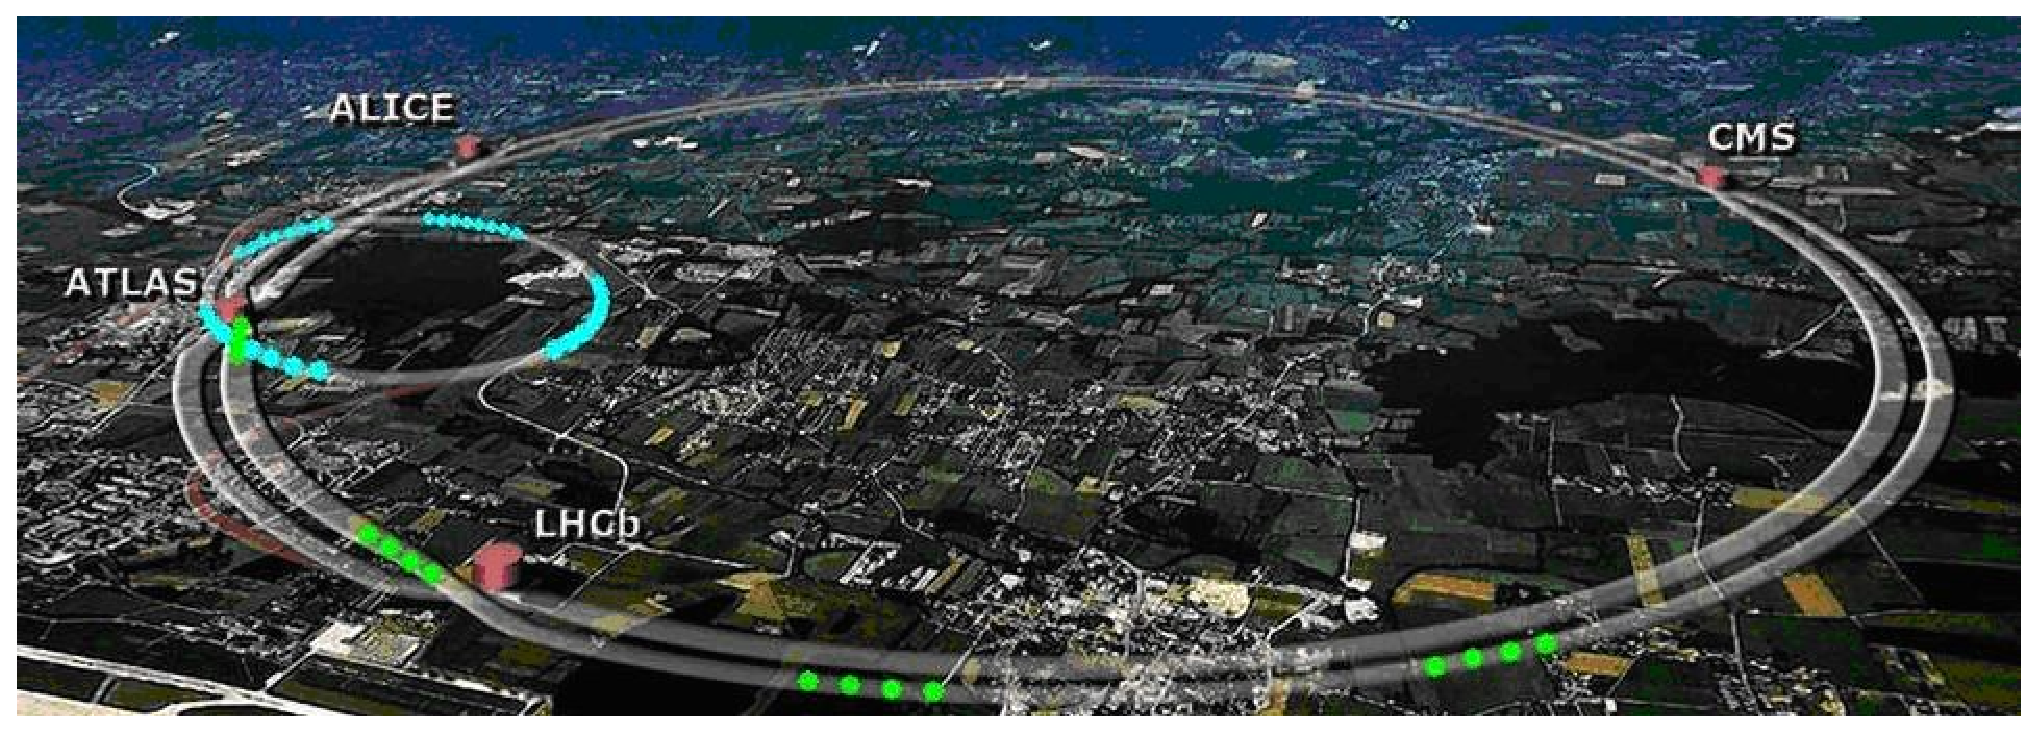
\includegraphics[width=13cm]{fig01.eps} %    ** if .eps don't need extension
\caption{LHC@CERN}\label{fig01}
\end{figure}



The phrase often used to summarize the mission of the LHC is, that
with the LHC we are going back in time very close to the Big Bang,
as close as about $10^{-10}$ seconds. In terms of length it represents
about $10^{-16}$ cm (compared to the dimensions of the Universe of about
$10^{28}$ cm). At this scale, the matter existed in a form of a ``soup''
made of the quarks and gluons, the Quark Gluon Plasma. The quarks
are objects protons and neutrons are made of, so the LHC represents
in a sense a huge extremely complicated microscope enabling the
study of the most basic elements of matter.

There are basically three major questions which scientists hope to
get answered with the help of the LHC.

\begin{itemize}
\item What is the origin of mass, why do elementary particles have
some weight? And why do some particles have no mass at all? At
present, we have no established answers to these questions. The
theory offering a widely accepted explanation, the Standard Model
[9], assumes the existence of a so-called Higgs boson, a key particle
undiscovered so far, although it was first hypothesized in 1964. One
of the basic tasks of the LHC is to bring an established statement
concerning the existence of the Higgs boson.

\item Where did all the anti-matter disappear? We are living in the
World where everything is made of matter. We suppose that at the
start of the Universe, equal amounts of matter and antimatter were
produced in the Big Bang. But during the early stages of the
Universe, an un-known deviation or in-equilibrium must have happened
resulting in the fact that in our world today, hardly any antimatter
is left.

\item What are the basic properties of the Quark-Gluon Plasma, the
state of the matter existing for a tiny period of time after the Big
Bang? Originally, we thought it would behave like a plasma, but the
latest scientific results including those delivered by the LHC
suggest that it behaves like a perfect liquid [2],
which is somewhat surprising for us.
\end{itemize}

From the four experiments analyzing the data from the LHC
collisions, ATLAS and CMS are the largest. They were nominally
designed to look for the Higgs boson but in fact these are general
purpose detectors for the study of all kinds of Physics phenomena at
the LHC  energy range. The LHCb is much smaller detector and its
mission is to study the asymmetry between matter and antimatter. The
ALICE  detector is a dedicated heavy ions detector to study the
properties of the Quark Gluon Plasma formed in the collisions of
lead ions  at the LHC energies. Although all these experiments are
designed for Particle Physics research, the scientific programs they
follow actually cross a border between Particle Physics,
Astrophysics and Cosmology.

Now, where the Computing Grid shows up in this scientific set-up?
The LHC is the world's largest particle accelerator. The protons and
lead ions are injected into the accelerator in bunches, in
counter-rotating beams. According to the original design proposal,
there should be 2808 bunches per a beam. Each bunch of protons
contains $10^{11}$ protons. the design beam energy is 7~TeV and the
design luminosity is $10^{34}\ $cm${}^{-2}$s${}^{-1}$. The bunch
crossing rate is 40~MegaHz and the proton collisions rate
$10^7-10^9$ Hz.

However, the new phenomena looked for by the scientists appear at a
rate of $10^{-5}$ Hz. So the physicists must analyze $10^{13}$
collision events/sec to have a chance to discover a New Physics
phenomenon. At present, the machine has not yet reached the full
number of bunches per beam and is operating at half of the
originally proposed energy, but the luminosity is getting rapidly to
the goal value. The LHC team has been increasing the number of
bunches gradually reaching 1380 bunches/beam at the time of writing.
The full beam energy will be reached in 2014, after one year of a
technical stop to arrange for this increase. The machine has already
beaten some world records which we will mention in section 5. Let us
just mention the one concerning the stored energy. In the end of
2010, the energy stored in the accelerator ring was about 28~MegaJoules (MJ).
At the target full intensity, this energy will
reach about 130~MJ which is an equivalent of 80~kg of the TNT.

In any case, the volume of data necessary to analyze to discover New
Physics was already in the original proposal estimated to be about
15 PetaBytes (PB, 1PB=1 million GB) per one data taking year. And
the number of the processor cores, CPUs, needed to process this
amount of data was estimated to be about 200 thousands. And here,
the concept of a distributed data management infrastructure comes
into the scenario, because there has not been any single computing
center within the LHC community/collaboration to offer so massive
computing resources, even not CERN. Therefore in 2002, the concept
of the Worldwide LHC Computing Grid (WLCG) [10] was launched to
build a distributed computing infrastructure to provide the
production and analysis environments for the LHC experiments.

In the present article, we give a short overview of the Grid
computing for the experiments at the LHC and the basics of the
mission of the WLCG.  Since we are members of the ALICE
collaboration, we will also describe some specific features of the
ALICE distributed computing environment.

In section 2, we will describe the architecture of the WLCG, which
consist of an agreed set of services and applications running on the
Grid infrastructures provided by the WLCG partners. In section 3, we
will mention some of the middleware services provided by the WLCG
which are used for the data access, processing, transfer and
storage. Although WLCG depends on the underlying Internet - computer
and communications networks, it is the special kind of software, so-called
middleware, that enables the user to access computers
distributed over the network. It is called ``middleware'' because it
sits between the operating systems of the computers and the Physics
applications that solve particular problems. In section 4, the
Computing model of the ALICE experiment will be briefly described.
It provides guide lines for the implementation and deployment of the
ALICE software and computing infrastructure over the resources
within the ALICE Grid and includes planning/estimates of the amount
of needed computing resources. Section 5
will be devoted to the ALICE-specific Grid services and the ALICE
Grid middleware AliEn. It is a set of tools and services which
represents an implementation of the ALICE distributed computing
environment integrated in the WLCG environment.  In section 6, an
overview will be given of the experience and performance of the WLCG
project and also of the ALICE Grid project in particular during the
real LHC data taking. The continuous operation of the LHC started in
November 2009.  When the data started to flow from the detectors,
the distributed data handling machinery was performing almost
flawlessly as a result of many years of a gradual development,
upgrades and stress-testing prior to the LHC startup. As a result of
the astounding performance of WLCG, a significant number of people
are doing analysis on the Grid, all the resources are being used up
to the limits and the scientific papers are produced with an
unprecedented speed within weeks after the data was recorded.

Section 7 contains a short summary and an outlook. This article is
meant to be a short overview of the facts concerning the Grid
computing for HEP experiments, in particular for the experiments at
the CERN LHC. The first one and half a year of the LHC operations
have shown that WLCG has built a true, well functioning distributed
infrastructure and the LHC experiments have used it to rapidly
deliver Physics results. The existing WLCG infrastructure has been
and will be continuously developing into the future absorbing and
giving rise to new technologies, like the advances in networking,
storage systems, middleware services and inter-operability between
Grids and Clouds.

%%%%%%%%%%%%%%%%%%% section 2 %%%%%%%%%%%%%%%%%%%%%%%%%%%%%%%%%%%%%%%%

\section{WLCG}

As mentioned in section 1, the LHC experiments are designed to
search for rare events with the signal/noise ratio as low
as $10^{-13}$. This Physics requires a study of enormous number of
pp and Pb-Pb collisions resulting in the production of data volumes
of more than 10 PetaBytes per one data taking year. The original
estimates elaborated when the LCG TDR [11] was put together were
about $\sim 15$~PetaBytes (PB) of new data each year which
translates into $\sim 200$ thousands of CPUs/processor cores and
45~PB of disk storage to keep the raw, processed and simulated data.

Nowadays, 200 thousands cores does not sound like much and one can
find them in large computer centers. 50~PB of a disk storage is
however not that common. In any case, at the time the LHC Computing
Grid was launched there was no single site within the LHC community
able to provide such computing power. So, the task of
processing the LHC data has been a distributed computing problem
right from the start whether the community liked it or not.

\subsection{WLCG mission}
%
The Worldwide LHC Computing Grid (WLCG) project [11] was launched in
2002 to provide a global computing infrastructure to store,
distribute and process the data annually generated by the LHC.
It integrates thousands of computers and storage systems
in hundreds of data centers worldwide, see Figure~\ref{fig02}. CERN
itself provides only about 20\% of the resources needed to manage
the LHC data. The rest is provided by the member states' national
computing centers and research network structures supported by
national funding agencies. The aim of the project is the
"collaborative resource sharing" between all the scientists
participating in the LHC experiments, which is the basic concept of
a Computing Grid as defined in [12]. The infrastructure is managed
and operated by a collaboration between the experiments and the
participating computer centers to make use of the resources no
matter where they are located.

%fig02
\begin{figure}[htb] % h-here, t-top, b-bottom
\centering
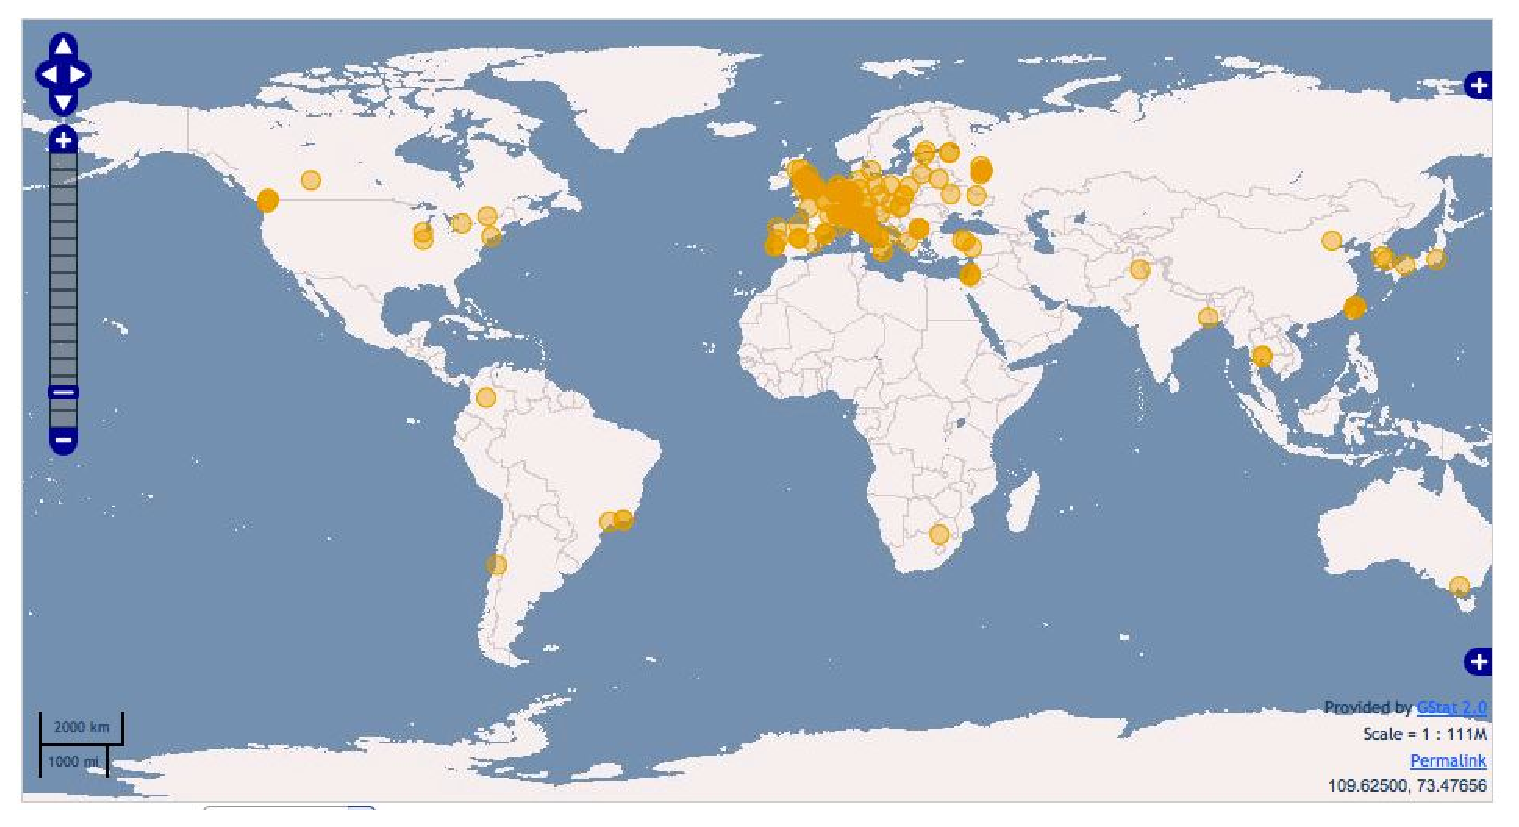
\includegraphics[width=13cm]{fig02.eps} %    ** if .eps don't need extension
\caption{Distribution of WLCG computing centers}\label{fig02}
\end{figure}



The collaboration is truly worldwide: it involves 35 countries on 5
continents and represents 49 funding agencies having signed the WLCG
Memorandum of Understanding on Computing (WLCG MoUC) [13]. The
distributed character has also a sociological aspect: although some
countries contribute more and some less into the whole
infrastructure according to their capabilities, a member of any
institution involved can access and analyze the LHC data from
his/her institute.

Currently, the WLCG integrates over 140 computing sites, more than
250 thousands CPU cores and over 150~PB of disk storage. It is now
the world's largest computing grid: the WLCG operates resources
provided by other collaborating grid projects: either the two main
global grids, EGI [14] and OSG [15], or by several regional or
national grids.

\subsection{Hierarchical (Tier) structure, the roles of different
Tier-sites}
%
The WLCG has a hierarchical structure based on the
recommendations of the project MONARC [16], see Figure~\ref{fig03}.
The individual participating sites are  classified according to their
resources and level of provided services into several categories
called Tiers. There is one Tier-0 site  which is CERN, then 11 Tier-1
centers, which are large computing centers with thousands of CPUs,
PBs of disk storage, tape storage  systems and 24/7 Grid support
service (Canada: TRIUMF, Germany: KIT/FZK, Spain: Port d'Informaci�
Cient�fica (PIC), France: IN2P3,  Italy: INFN, Nordic countries:
Nordic Datagrid Facility (NDGF), Netherlands: NIKHEF/SARA, Taipei:
ASGC, United Kingdom: GridPP, USA: Fermilab-CMS and USA: BNL ATLAS).
Then there are currently about 140 Tier-2 sites covering most of the
globe. The system also recognizes Tier-3 centers, which are small
local computing clusters at universities or research institutes.

%fig03
\begin{figure}[htb] % h-here, t-top, b-bottom
\centering
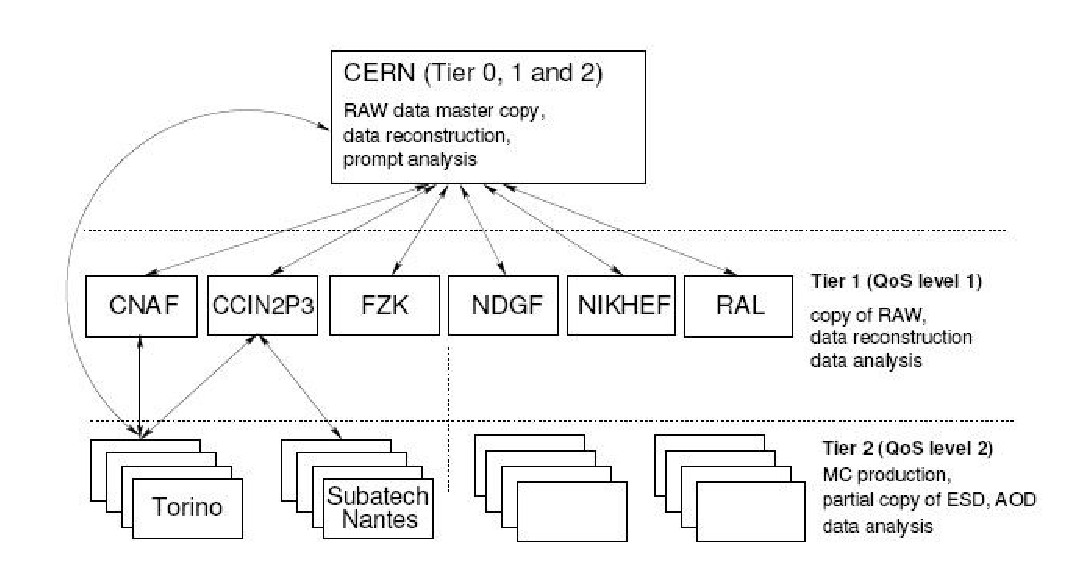
\includegraphics[width=13cm]{fig03.eps} %    ** if .eps don't need extension
\caption{Schema of the hierarchical Tier-like structure of
WLCG}\label{fig03}
\end{figure}




The raw data recorded by the LHC experiments (raw data) is shipped
at first to the CERN Computing Center (CC) through dedicated links.
CERN Tier-0 accepts data at average of 2.6~GBytes(GB)/s with peaks
up to 11 GB/s. At CERN, the data is archived in the CERN tape system
CASTOR [12] and goes through the first level of processing - the
first pass of reconstruction. The raw data is also replicated to the
Tier-1 centers, so there are always 2 copies of the raw data files.
CERN serves data at average of 7 GB/s with peaks up to 25 GB/s [17].
The Tier-0 writes on average 2~PB of data per month to tape in pp
running, and double that in the 1 month of Pb-Pb collisions, (cf.
Figures~\ref{fig04},\ref{fig05}).


%fig04
\begin{figure}[htb] % h-here, t-top, b-bottom
\centering
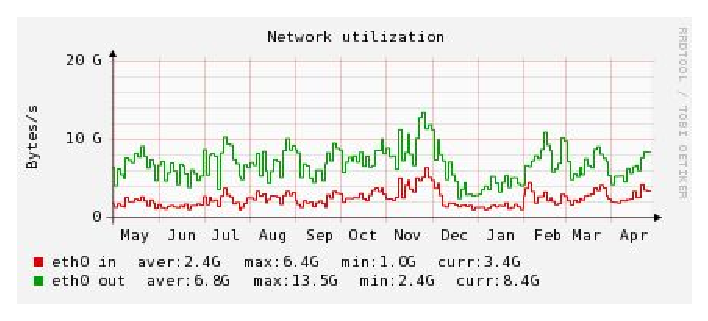
\includegraphics[width=13cm]{fig04.eps} %    ** if .eps don't need extension
\caption{CERN Tier-0 Disk Servers (GB/s), 2010/2011}\label{fig04}
\end{figure}



%fig05
\begin{figure}[htb] % h-here, t-top, b-bottom
\centering
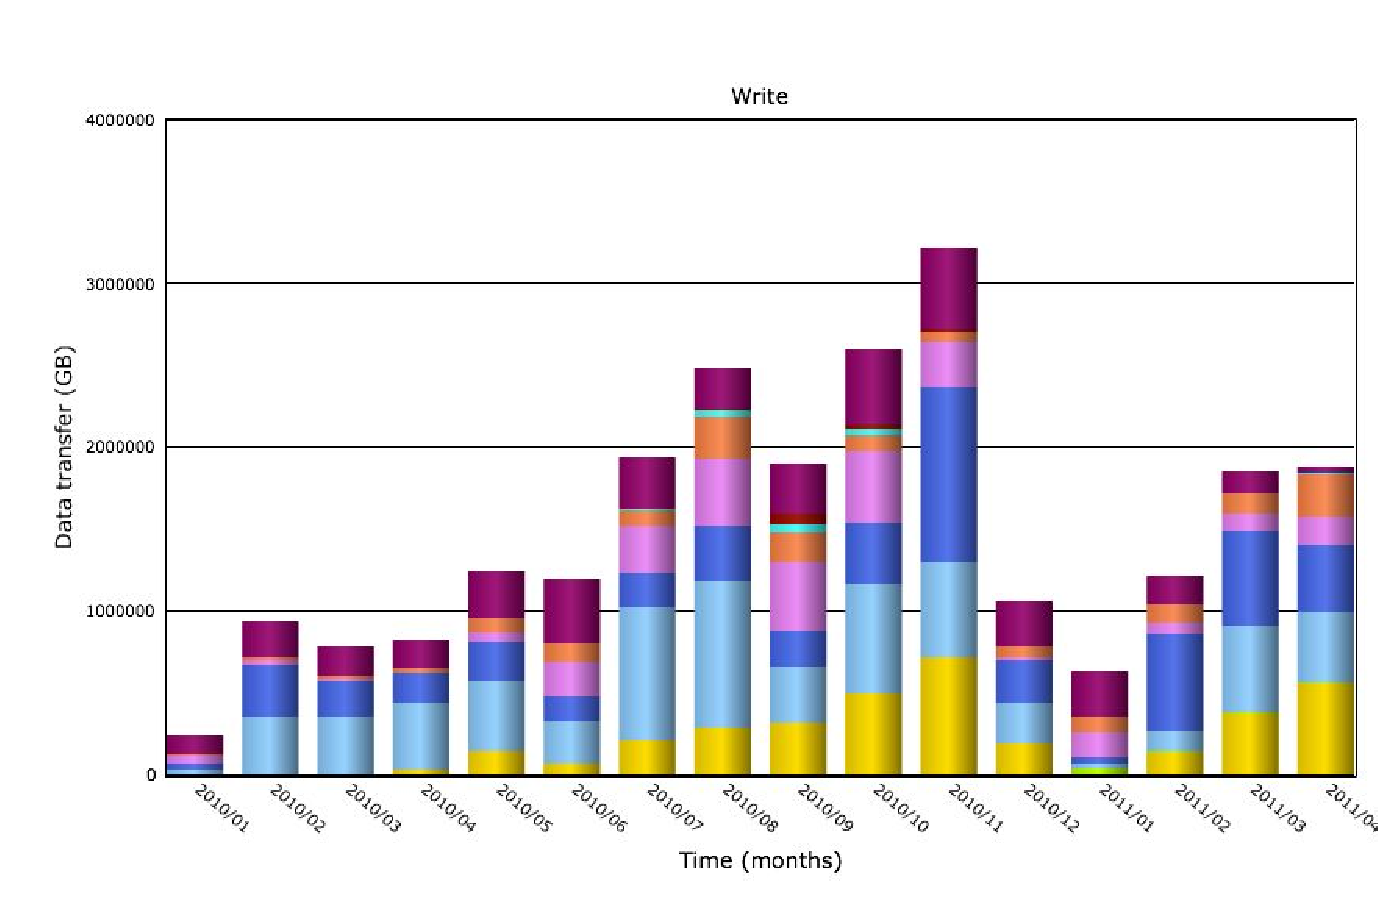
\includegraphics[width=13cm]{fig05.eps} %    ** if .eps don't need extension
\caption{Data written to tape at the CERN Tier-0
(GB/month)}\label{fig05}
\end{figure}


At Tier-1 centers, the raw data replicas are permanently stored as
mentioned before and several passes of the data re-processing are
performed. This multiple-stage data re-processing is performed using
methods to detect interesting events through the processing
algorithms, as well as improvements in detector calibration, which
are in continuous evolution and development. Also, the scheduled
analysis productions as well as some of the end user analysis jobs
are performed at Tier-1s.

Tier-2 centers  (more than 130 in the WLCG, integrated within 68
Tier-2 federations) are supposed to process simulation (Monte Carlo
simulations of the collision events in the LHC detectors) and
end-user analysis jobs. The load of simulations needed to correctly
interpret the LHC data is quite sizeable, close to the raw data
volume. The number of end users regularly using the WLCG
infrastructure to perform analysis is larger than expected in the
beginning of the LCG project, it varies from about 250 to 800 people
depending on the experiment. This is certainly also a result of the
experiments' effort to hide the complexity of the Grid from the
users and make the usage as simple as possible. Tier-2 sites deliver
more than 50\% of the total CPU power within the WLCG, see
Figure~\ref{fig06}.

%fig06
\begin{figure}[htb] % h-here, t-top, b-bottom
\centering
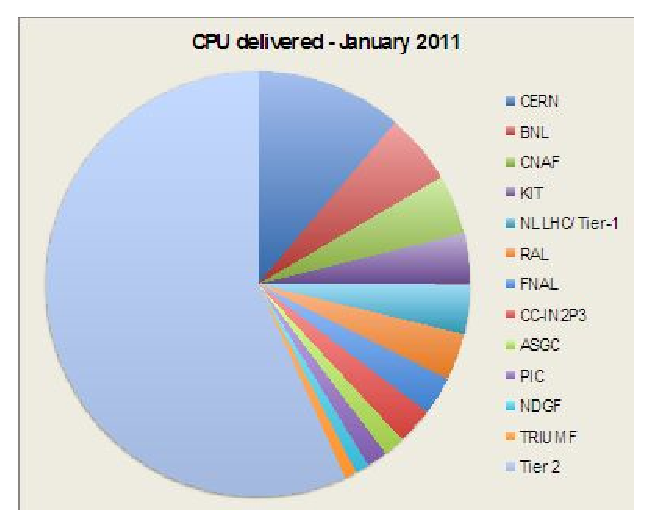
\includegraphics[width=13cm]{fig06.eps} %    ** if .eps don't need extension
\caption{CPU resources in WLCG, January 2011. More than 50\% was
delivered by Tier-2s.}\label{fig06}
\end{figure}



\subsection{Network}
%
The sustainable operation of the data storing and processing
machinery would not be possible without a reliable network
infrastructure. In the beginning of the WLCG project there were
worries that the infrastructure would not be able to transfer the
data fast enough. The original estimates of the needed rate were
about 1.3~GB/s from CERN to external Tiers. After the years spent
with building the backbone of the WLCG network, CERN
is able to reach rates about 5~GB/s to Tier-1s, see
Figure~\ref{fig07}.

%fig07
\begin{figure}[htb] % h-here, t-top, b-bottom
\centering
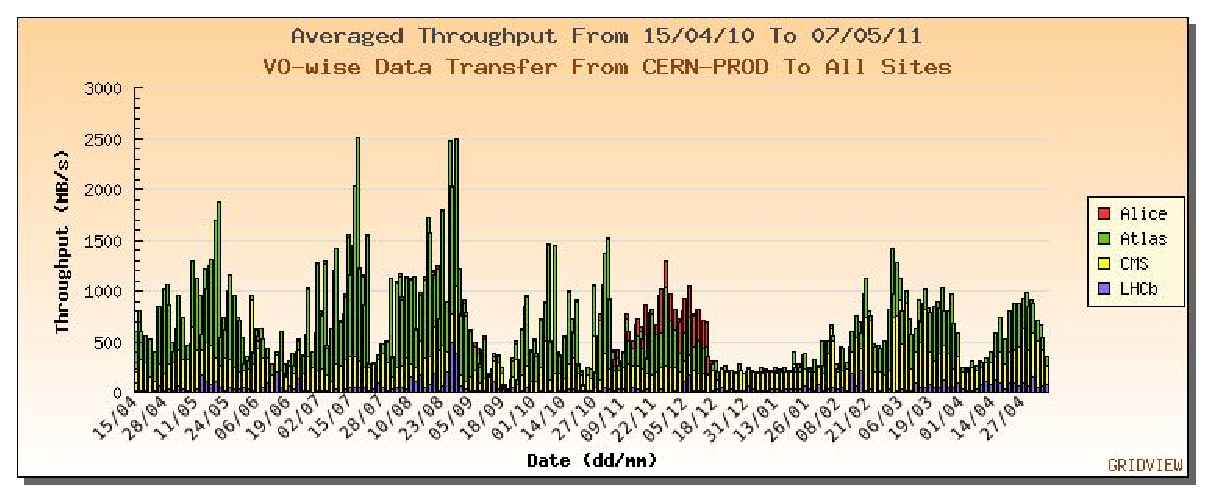
\includegraphics[width=13cm]{fig07.eps} %    ** if .eps don't need extension
\caption{Average throughput from CERN to all Tiers}\label{fig07}
\end{figure}


The WLCG networking relies on the Optical Private Network (OPN)
backbone [18], see Figure~\ref{fig08}, which is composed of dedicated
connections between CERN Tier-0 and each of the Tier1s, with the
capacity of 10~Gbit/s each. The original connections proliferated
into duplicates or backroutes making the system considerably
reliable. The OPN is then interconnected with national network
infrastructures like the GEANT [19] in Europe or the US-LHCNet [20]
and all the National Research and Education Networks (NRENs) in
other countries.

%fig08
\begin{figure}[htb] % h-here, t-top, b-bottom
\centering
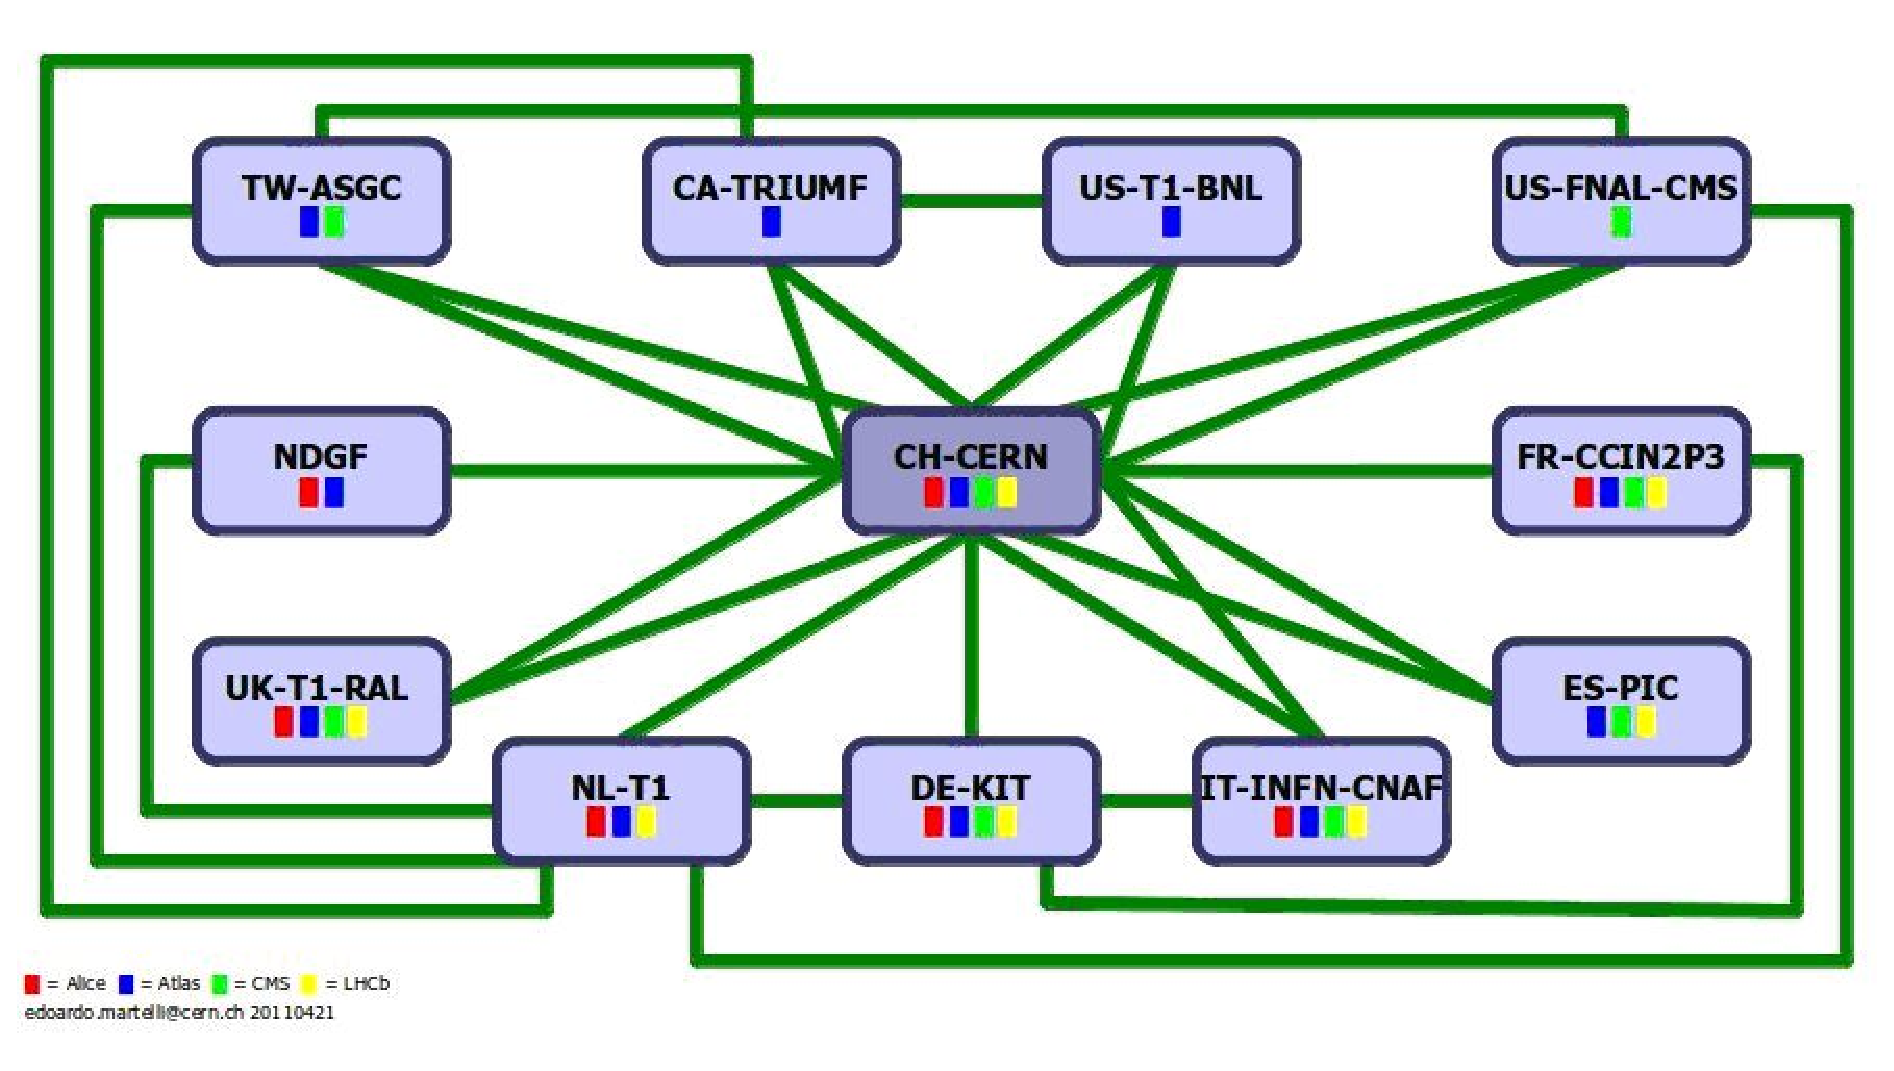
\includegraphics[width=13cm]{fig08.eps} %    ** if .eps don't need extension
\caption{LHCOPN}\label{fig08}
\end{figure}


There exists a concept of so-called LHCONE [17], which should enable
a good connectivity of Tier-2s and Tier-3s to the Tier-1s without
overloading the general purpose network links. It will extend and
complete the existing OPN infrastructure to increase the
interoperability of all the WLCG sites.

\subsection{Data and Service challenges}
%
As we will describe in section~6, the WLCG data management
worked almost flawlessly when the real data started
to flow from the detectors in the end of 2009. But this was not just
a happy coincidence. There were over 6 years of continuous testing
of the infrastructure performance. There was a number of independent
experiments' so-called Data Challenges which started in 2004, when
the "artificial raw" data was generated in the Monte Carlo
productions and then processed and managed as if it was the real raw
data. Then there was a series of WLC Service Challenges also
starting in 2004, with the aim to demonstrate WLCG services aspects:
data management, scaling of job workloads, security incidents,
interoperability, support processes and all was topped with data
transfers exercise lasting for weeks. The last test was the Service
Challenge STEP'09 including all experiments and testing full
computing models. Also, the cosmic data taking which started in 2008
has checked the performance of the data processing chain on a
smaller scale.

Currently, whether the data taking is going on or not, the network,
especially the OPN, and the sites are under continuous checking:
there  are automatically generated test jobs periodically sent over
the infrastructure to test the availability and functioning of the
network and on-site services.

\subsection{Concluding remarks}
%
The WLCG integrates and operates resources distributed all over the
world and its task is to make all these resources accessible and
usable for the LHC experiments to distribute, archive and process
the data produced by the LHC. This task is done using a specialized
software called ``middleware'' because it sits between the operating
systems of the computers at the WLCG sites and the Physics
applications software used for the reconstruction, analysis and
simulation of the LHC data (or any other application software
layer). The middleware is a collection of protocols, agents and
programs/services which we describe in the following section.

%%%%%%%%%%%%%%%%%%%%%%%%% section 3 %%%%%%%%%%%%%%%%%%%%%%%%%%%%%%%%%%%%%%%%%%%%%%%%%%%%%%%%%%%%%

\section{Middleware}

As we already mentioned, the Worldwide LHC Computing Grid is a
distributed computing infrastructure that spans over 5 continents
managing resources distributed across the world (for funding,
operability and access reasons). The resources operated by the WLCG
belong either to the two main global grids, EGI [14] and OSG [15], or
to other collaborating regional or national grids. To make this
diverse variety of resources globally available for all the WLCG
users, the WLCG has been developing its own middleware, a software
layer that ``brings all the resources together'': a collection of
programs, services and protocols to manage and operate the entire
WLCG infrastructure (see Figure~\ref{fig09}).

%fig09
\begin{figure}[htb] % h-here, t-top, b-bottom
\centering
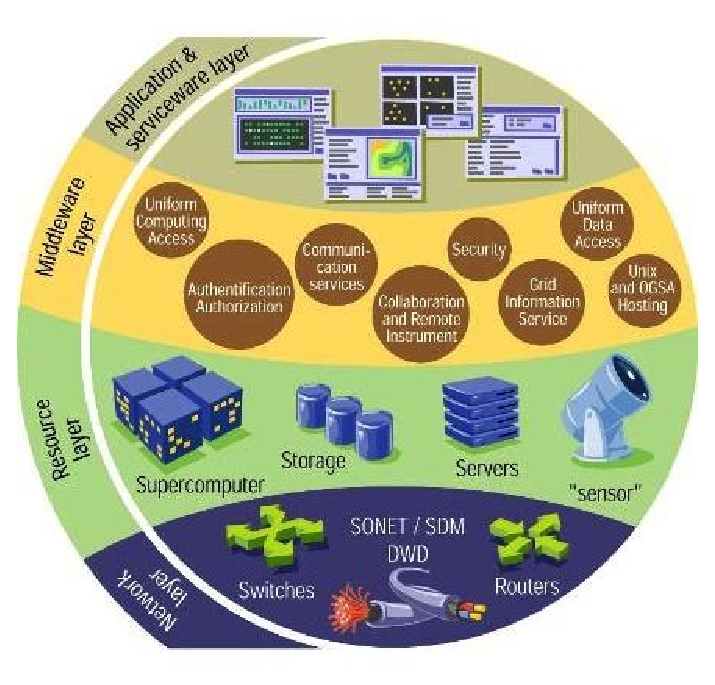
\includegraphics[width=13cm]{fig09.eps} %    ** if .eps don't need extension
\caption{Grid Layers}\label{fig09}
\end{figure}



\subsection{Overview of Grid services}
%
The WLCG middleware is a complex suite of packages which includes
(see also Figure~\ref{fig10}):

\begin{itemize}
\item Data Management Services:
%
\begin{itemize}
\item Storage Element
\item File Catalogue Service
\item Grid file access tools
\item File Transfer Service
\item GridFTP service
\item Database and DB Replication Services
\item POOL Object Persistency Service
\end{itemize}
%
\item Security Services:
%
\begin{itemize}
\item Certificate Management Service
\item Virtual Organization [21] Management Registration Service (VOMRS)
\item Authentication and Authorization Service (the X509 infrastructure)
\end{itemize}
%
\item Job Management Services:
%
\begin{itemize}
\item Compute Element
\item Workload Management
\item Service VO Agent Service
\item Application Software Install Service
\end{itemize}
%
\item Information Services:
%
\begin{itemize}
\item Accounting Service
\item Site Availability Monitor
\item Monitoring tools: experiment dashboards; site monitoring
\end{itemize}
%
\end{itemize}

%fig10
\begin{figure}[htb] % h-here, t-top, b-bottom
\centering
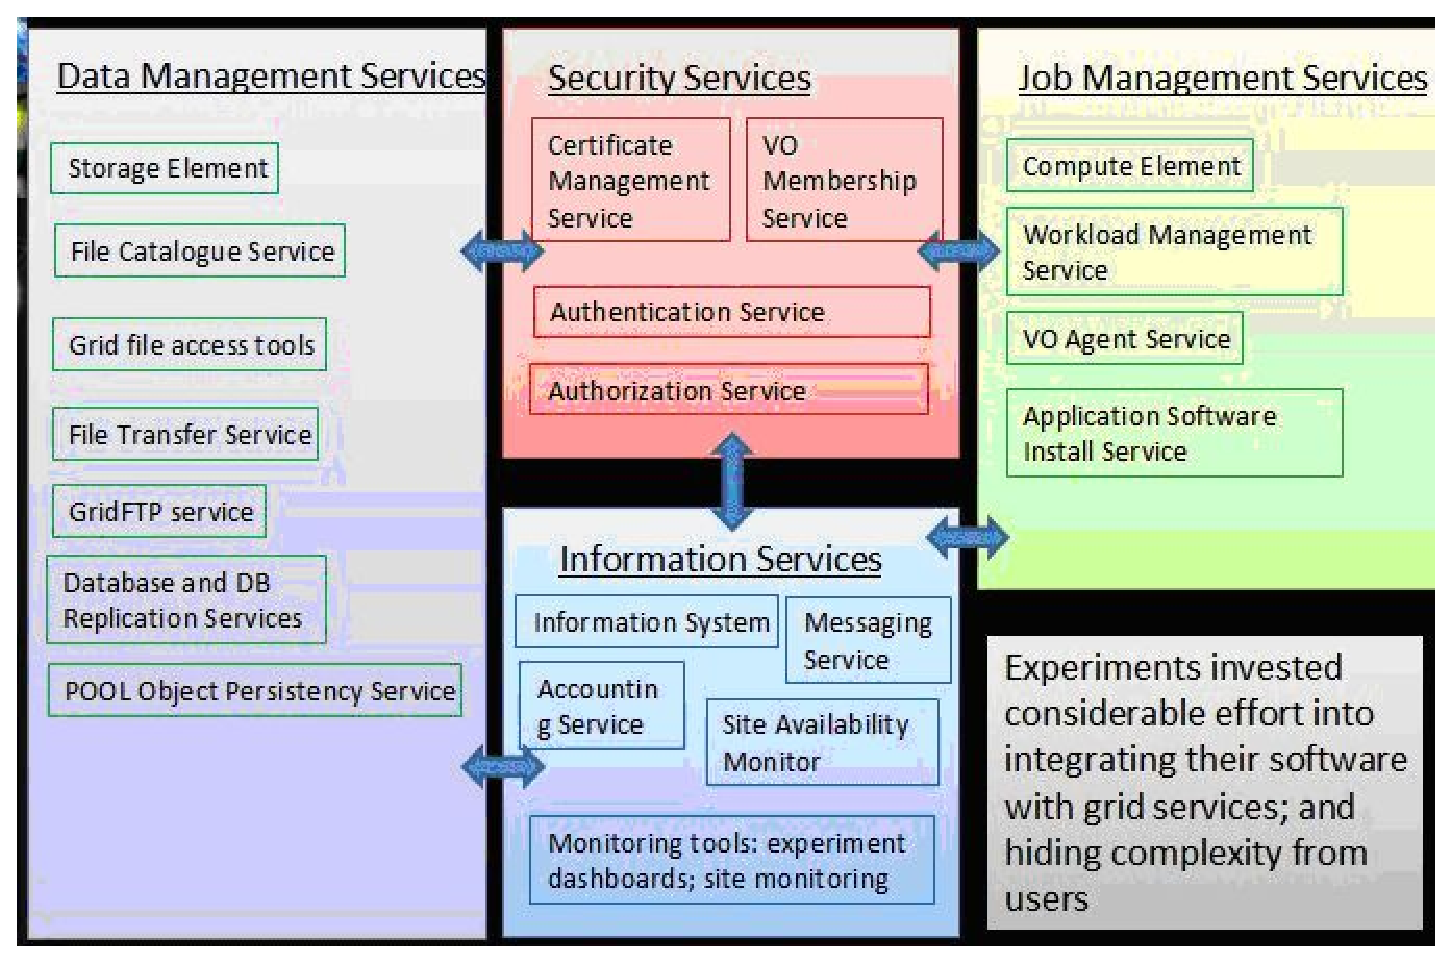
\includegraphics[width=13cm]{fig10.eps} %    ** if .eps don't need extension
\caption{Schema of Grid services}\label{fig10}
\end{figure}



The WLCG middleware has been built and further developed using and
developing some packages produced by other projects including, e.g.:
%
\begin{itemize}
\item EMI (European Middleware Initiative) [22], combining the key
middleware providers of ARC, gLite, UNICORE and dCache
\item Globus Toolkit [23] developed by the Globus Alliance
\item OMII from the Open Middleware Infrastructure Institute [24]
\item Virtual Data Toolkit [25]
\end{itemize}

\subsection{Experiments' specific developments}
%
All the LHC experiments created their own specific Computing models
summarized in the individual Computing Technical Design Reports (TDRs).
They do not rely only on the WLCG-provided middleware packages
but are also developing
some specific components tailored to better comply with their
Computing models.

For example the ALICE experiment, has developed a grid middleware
suite AliEn [26] (AliCE Environment), which provides a single
interface for a transparent access to computing resources for the
ALICE community. AliEn consists of a collection of components and
services which will be described in the next section. AliEn together
with selected packages of the WLCG-provided middleware gives a
complete framework to the ALICE community to manage and process the
data produced by the LHC according to the ALICE Computing model.

All the LHC experiments invested a considerable effort into
shielding the users from the underlying complexity of the Grid
machinery trying to provide relatively simple entry points into the
Grid. This effort has payed off and is reflected in a considerable
number of physicists actually using the WLCG for their analysis.

\subsection{Selected WLCG-provided services}
%
In the following section, we will describe as an example the
Computing model of the ALICE experiment. The WLCG services used in
this model include the Computing Element (CE), the Storage Element
(SE) and the VOBOX.

\subsubsection{Computing Element}
%
The Computing Element (CE) [27] is a middleware component/grid
service providing an entry point to a grid site. It authenticates
users and submits jobs to Worker Nodes (WN), aggregates and
publishes information from the nodes. It includes a generic
interface to the local cluster called Grid Gate (GG), Local Resource
Management System (LRMS) and the collection of Worker Nodes.

The submission of jobs to CEs is performed by the Workload
Management System (WMS) [28], a middleware component/grid service,
that also monitors jobs status and retrieves their output. WLCG
(gLite) CE is a computing resource access service using standard
grid protocols. To improve the performance, the CREAM (Computing
Resource Execution And Management) Computing Element [29] has
replaced the gLite-CE in production since about 2009. It is a
simple, lightweight service for job management operation at the
Computing Element level. CREAM-CE accepts job submission requests
(described with the same files as used for the Workload Management
System) and other job management requests like e.g. job monitoring.
CREAM-CE can be used by a generic client, e.g. an end-user willing
to directly submit jobs to a CREAM-CE.

\subsubsection{Storage Element (XRootD)}
%
The Storage Element (SE) [30] provides storage place and access for
data. Important variables apart from available storage space,
read/write speeds and bandwidth concern reliability against
overload, percentage of failed transfers from/to SE and percentage
of lost/corrupted files.

WLCG (gLite) provides dCache [31] and DPM [32] storage management
tools used by the LHC experiments. However within the ALICE
infrastructure, the preferred storage manager is the Scalla/XRootD
package [33] developed within a SLAC [34] - CERN collaboration
(originally, it was a common project of SLAC and INFN [35]). After
CERN got involved, the XRootD was bundled in ROOT [36] as a generic
platform for distributed data access, very well suited for the LHC
data analysis.

The primary goal has been the creation of data repositories with no
reasonable size limit, with high data access performance and linear
scaling capabilities. The framework is a fully generic suite for
fast, low latency and scalable data access, which can serve any kind
of data, organized as a hierarchical filesystem-like namespace,
based on the concept of directory.

``xrootd'' is just the name of the data access daemon. Although
fundamental, it is just a part of the whole suite. The complete
suite is called Scalla/XRootD, Scalla meaning Structured Cluster
Architecture for Low Latency Access.

The manager exhibits important features including:
%
\begin{itemize}
\item High speed access to experimental data
\item High transaction rate with rapid request dispersement (fast
open, low latency)
\item Write once read many times processing mode
\item Fault tolerance (if servers go, the clients do not die)
\item Fault tolerance (able to manage in realtime distributed
replicas)
\item Integrated in ROOT
\end{itemize}

From the site administrator point, the following features are
important:
\begin{itemize}
\item  No database requirements (no backup/recovery issues, high
performance)
\item Resources gentle, high efficiency data server (low
CPU/byte overhead, small memory footprint)
\item  Simple installation
\item Configuration requirements scale linearly with site complexity
\item No 3rd party software needed (avoids messy dependencies)
\item Low administration costs
\item Self-organizing servers remove need for
configuration changes in big clusters
\end{itemize}

Additional features:
\begin{itemize}
\item Generic Mass Storage System Interface (HPSS, CASTOR, etc)
\item Full POSIX access
\item Server clustering for scalability, supports large number of
clients from a small number of servers
\item Up to 262000 servers per cluster
\item High WAN data access efficiency (exploit the throughput of
modern WANs for direct data access, and for copying files as well)
\end{itemize}

\subsubsection{VOBOX}
%
The VOBOX [37] is a standard WLCG service developed in 2006 in order
to provide the LHC experiments with a place where they can run their
own specific agents and services, whenever the WLCG middleware still
does not provide the required functionality. In addition, it
provides the file system access to the experiment software area.
This area is share between VOBOX and the Worker Nodes at the given
site.  VOBOX is installed at the WLCG sites on dedicated machines
and its installation is mandatory for sites to enter the grid
production (it is an "entry door" for a site to the WLCG
environment). The access to the VOBOX is restricted to the Software
Group Manager (SGM) of the given Virtual Organization. Since 2008,
this WLCG service has been VOMS-aware [34]. In the following
section, we will describe the services running on the VOBOX machines
reserved at a site for the ALICE computing.

%%%%%%%%%%%%%%%%%%%% section 4 %%%%%%%%%%%%%%%%%%%%%%%%%%%%%%%%%%%%%%%%%%%%%%%%%%%%%%

\section{ALICE Computing model}

In this section, we will briefly describe the computing model of the
ALICE experiment [38].

ALICE (A Large Ion Collider Experiment) [5] is a dedicated heavy-ion
(HI) experiment at the CERN LHC which apart from the HI mission has
also its proton-proton (pp) Physics program. Together with the other
LHC experiments, ALICE has been successfully taking and processing
pp and HI data since the LHC startup in November 2009. During the pp
running, the data taking rate has been up to 500 MB/s while during
the HI running the data was taken with the rate up to 2.5 GB/s. As
was already mentioned, during 2010 the total volume of data taken by
the all LHC experiments reached 15~PB, which corresponds to 7~months
of the pp running and 1 month of the HI running (together with
4~months of an LHC technical stop for maintenance and upgrades this
makes up for one standard data taking year (SDTY)).

The computing model of ALICE relies on the ALICE Computing Grid, the
distributed computing infrastructure based on the hierarchical Tier
structure as described in section 2.  ALICE has developed over the
last 10 years a distributed computing environment and its
implementation: the Grid middleware suite AliEn (AliCE Environment)
[26], which is integrated in the WLCG environment. It provides a
transparent access to computing resources for the ALICE community
and will be described in the next section.

\subsection{Raw data taking, transfer and registration}
%
The ALICE detector consists of 18~subdetectors that interact with
5~online systems [5]. During data taking, the data is read out by
the Data Acquisition (DAQ) system as raw data streams produced by
the subdetectors, and is moved and stored over several media. On
this way, the raw data is formatted, the events (data sets
containing information about individual pp or Pb-Pb collisions) are
built, the data is objectified in the ROOT [36] format and then
recorded on a local disk. During the intervals of continuous data
taking called runs, different types of data sets can be collected of
which the so-called PHYSICS runs are those substantial for Physics
analysis. There are also all kinds of calibration and other
subdetectors' testing runs important for the reliable subsystems
operation.

ALICE experimental area (called Point2 (P2)) serves as an
intermediate storage: the final destination of the collected raw
data is the CERN Advanced STORage system (CASTOR) [39], the permanent
data storage (PDS) at the CERN Computing center. From Point2, the
raw data is transferred to the disk buffer adjacent to CASTOR at
CERN (see Figure~\ref{fig11}). As mentioned before, the transfer
rates are up to 500 MB/s for the pp and up to 2.5 GB/s for the HI
data taking periods.

%fig11
\begin{figure}[htb] % h-here, t-top, b-bottom
\centering
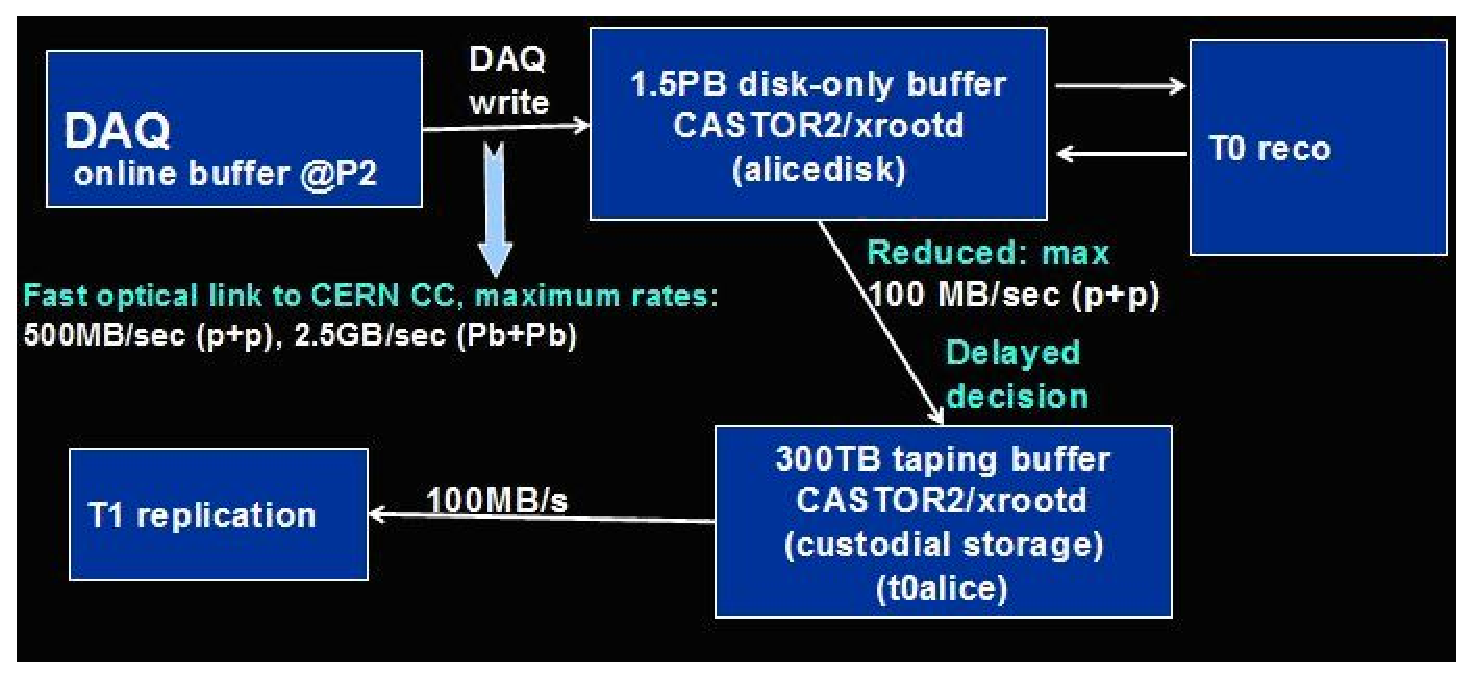
\includegraphics[width=13cm]{fig11.eps} %    ** if .eps don't need extension
\caption{Data processing chain}\label{fig11}
\end{figure}



After the migration to the CERN Tier-0, the raw data is registered
in the AliEn catalogue [26] and the data from PHYSICS runs is
automatically queued for the Pass1 of reconstruction, the first part
of the data processing chain, which is performed at the CERN Tier-0.
After the registration in AliEn, the data from PHYSICS runs is also
automatically queued for the replication to external Tier-1s (see
Figure~\ref{fig11}). It may happen that the replication is launched
and finished fast and the data goes through the first processing at
a Tier-1.

The mentioned automated processes are a part of a complex set of
services deployed over the ALICE Computing Grid infrastructure. All
the involved services are continuously controlled by automating
procedures reducing to a minimum the human interaction. The Grid
monitoring environment adopted and developed by ALICE, the
Java-based MonALISA (MONitoring Agents using Large Integrated
Services Architecture) [40], uses decision-taking automated agents
for management and control of the Grid services. For monitoring of
raw data reconstruction passes see [41].

The automatic reconstruction is typically completed within a couple
of hours after the end of the run (EOR). The output files from the
reconstruction are registered in AliEn and are available on the Grid
(stored and accessible within the ALICE distributed storage pool)
for further processing.


\subsection{Multiple reconstruction}
%
In general, the ALICE computing model for the pp data taking is
similar to that of the other LHC experiments. Data is automatically
recorded and then reconstructed quasi online at the CERN Tier-0
facility. In parallel, data is exported to the different external
Tier-1s, to provide two copies of the raw data, one stored at the
CERN CASTOR and another copy shared by all the external Tier-1s.

For HI (Pb-Pb) data taking this model is not viable, as data is
recorded at up to 2.5~GB/s.  Such a massive data stream would
require a prohibitive amount of resources for quasi real-time
processing. The computing model therefore requires that the HI data
reconstruction at the CERN Tier-0 and its replication to the Tier-1s
be delayed and scheduled for the period of four months of the LHC
technical stop and only a small part of the raw data (10-15\%) be
reconstructed for the quality checking. In reality, comparatively
large part of the HI data (about 80\%) got reconstructed and
replicated in 2010 before the end of the data taking due to
occasional lapses in the LHC operations and much higher quality of
the network infrastructure than originally envisaged.

After the first pass of the reconstruction, the data is usually
reconstructed subsequently more times (up to 6-7 times) for better
results at Tier-1s or Tier-2s . Each pass of the reconstruction
triggers a cascade of additional tasks organized centrally like
Quality Assurance (QA) processing trains and a series of different
kinds of analysis trains described later. Also, each reconstruction
pass triggers a series of the Monte Carlo simulation productions.
All this complex of tasks for a given reconstruction pass is
launched automatically as mentioned before.

\subsection{Analysis}
%
The next step in the data processing chain is then the analysis.
There are two types of analysis: a scheduled analysis organized
centrally and then the end-user, so-called chaotic analysis. Since
processing of the end-user analysis jobs often brings some problems
like a high memory consumption (see Figure~\ref{fig12}) or unstable
code, the scheduled analysis is organized in the form of so called
analysis trains (see [42]). The trains absorb up to 30 different
analysis tasks running in succession with one data set read and with
a very well controlled environment. This helps to consolidate the
end-user analysis.

%fig12
\begin{figure}[htb] % h-here, t-top, b-bottom
\centering
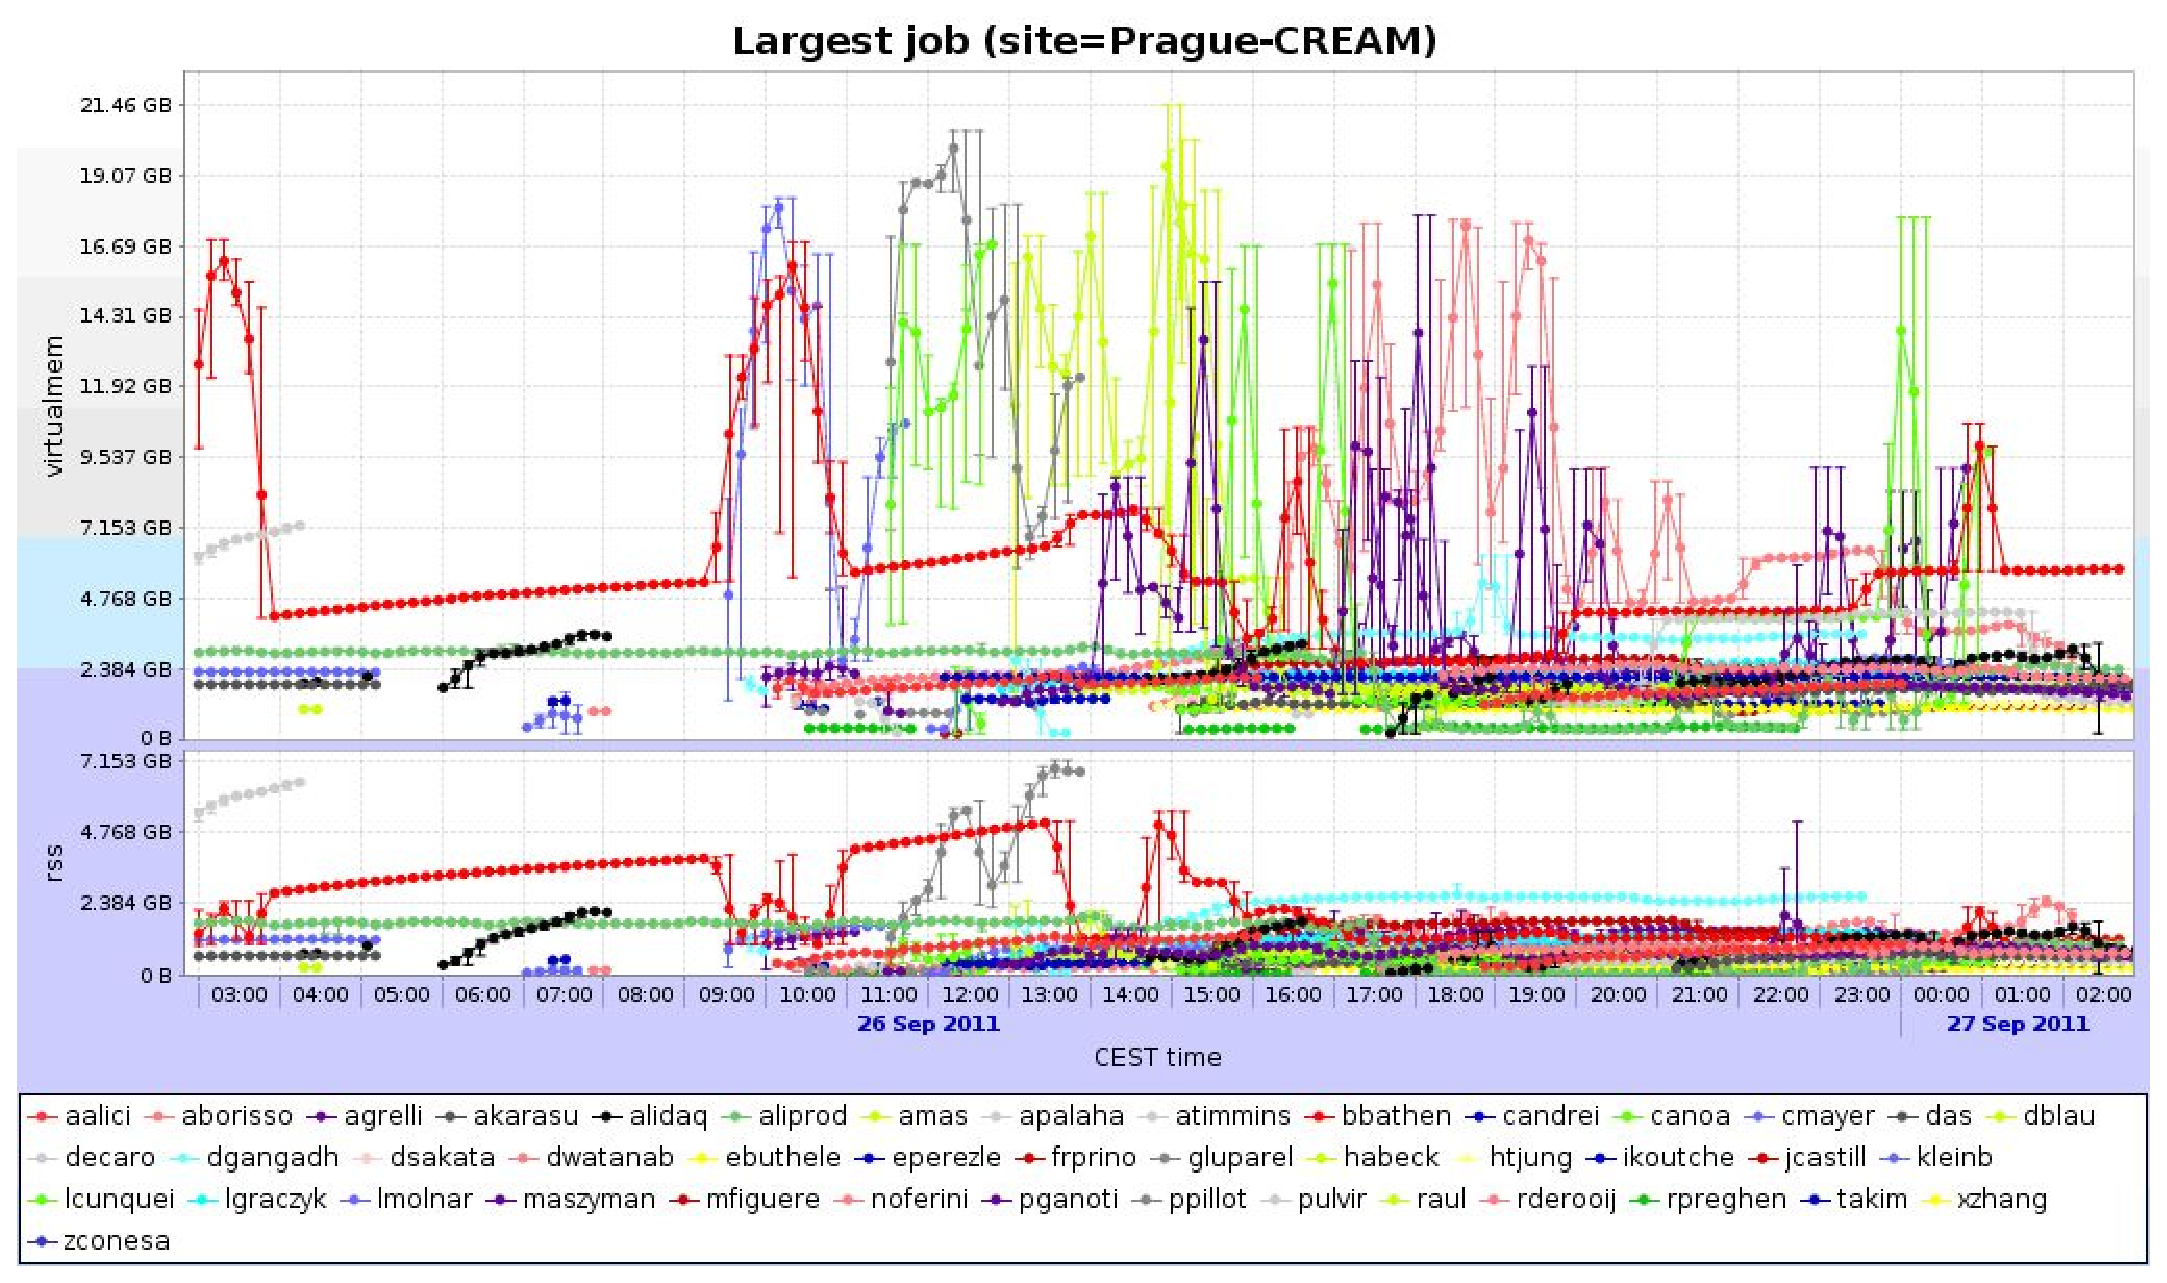
\includegraphics[width=13cm]{fig12.eps} %    ** if .eps don't need extension
\caption{End-user analysis memory consumption: peaks in excess of
20~GB}\label{fig12}
\end{figure}


The computing model assumes that the scheduled analysis will be
performed at Tier-1 sites, while the chaotic analysis and simulation
jobs will be performed at Tier-2s. The experience gained during the
numerous Data Challenges, the excellent network performance, the
stable and mature Grid middleware deployed over all sites and the
conditions at the time of the real data taking in 2010/2011
progressively replaced the original hierarchical scenario by a more
``symmetric'' model often referred to as the ``cloud model''.

\subsection{Simulations}
%
As already mentioned, ever since the start of building the ALICE
distributed computing infrastructure, the system was tested and
validated with increasingly massive productions  of Monte Carlo (MC)
simulated events of the LHC collisions in the ALICE detector. The
simulation framework [43] covers the simulation of primary collisions
and generation of the emerging particles, the transport of particles
through the detector, the simulation of energy depositions (hits) in
the detector components, their response in form of so called
summable digits, the generation of digits from summable digits with
the optional merging of underlying events and the creation of raw
data. Each raw data production cycle triggers a series of
corresponding MC productions (see [44]). As a result, the volume of
data produced during the MC cycles is usually in excess of the
volume of the corresponding raw data.

\subsection{AliRoot}
%
The ALICE software framework for reconstruction, simulation and
analysis of the data, AliRoot [45], has been under a steady
development since 1998. Typical use cases include detector
description, events generation, particle transport, generation of
``summable digits'', event merging, reconstruction, particle
identification and all kinds of analysis tasks. AliRoot uses the
ROOT [36] system as a foundation on which the framework for
simulation, reconstruction and analysis is built. The Geant3 [46] or
FLUKA [47] packages perform the transport of particles through the
detector and simulate the energy deposition from which the detector
response can be simulated. Except for large existing libraries, such
as Pythia6 [48] and HIJING [49], and some remaining legacy code,
this framework is based on the Object Oriented programming paradigm
and is written in C++.

AliRoot is constituted by a large amount of files, sources,
binaries, data and related documentation. Clear and efficient
management guidelines are vital if this corpus of software should
serve its purpose along the lifetime of the ALICE experiment. The
corresponding policies are described in [50].  For understanding and
improvement of the AliRoot performance, as well as for understanding
the behavior of the ALICE detectors, the fast feedback given by the
offline reconstruction is essential.

\subsection{Data types}
%
To complete the description of the ALICE data processing chain, we
will mention the different types of data files produced at different
stages of the chain (see Figure~\ref{fig13}).

As was already mentioned, the data is delivered by the Data
Acquisition system in a form of raw data in the ROOT format. The
reconstruction produces the so-called Event Summary Data (ESD), the
primary container after the reconstruction. The ESDs contain
information like run and event numbers, trigger class, primary
vertex, arrays of tracks/vertices, detector conditions. In an ideal
situation following the computing model, the EODs should be of 10\%
size of the corresponding raw data files.

The subsequent data processing provides so called Analysis Object
Data (AOD), the secondary processing product, which are data objects
containing more skimmed information needed for final analysis.
According to the Computing model, the size of AODs should be 2\% of
the raw data file size. Since it is difficult to squeeze all the
information needed for the Physics results in such small data
containers, this limit was not yet fully achieved.

%fig13
\begin{figure}[htb] % h-here, t-top, b-bottom
\centering
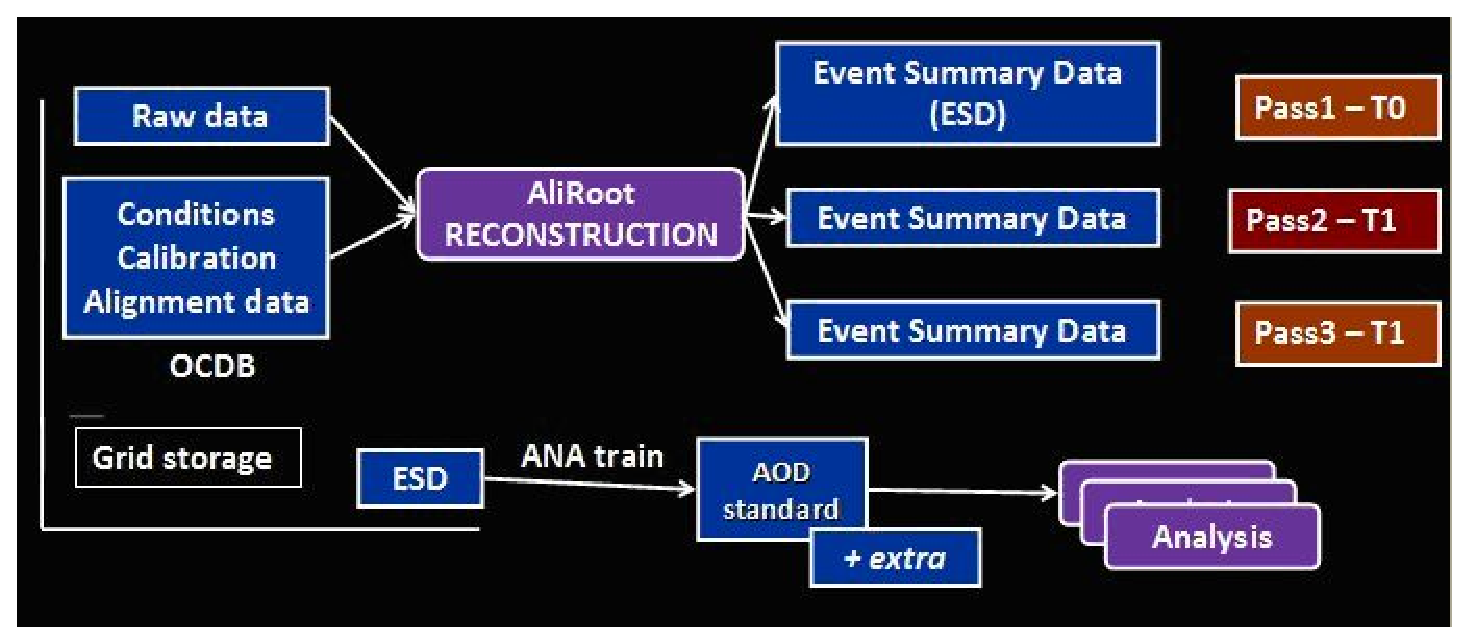
\includegraphics[width=13cm]{fig13.eps} %    ** if .eps don't need extension
\caption{Data types produced in the processing chain}\label{fig13}
\end{figure}


\subsection{Resources}
%
The ALICE distributed computing infrastructure has evolved from a
set of about 20 computing sites into a global world-wide system of
distributed resources for data storage and processing. As of today,
this project is made of over 80 sites spanning 5 continents (Africa,
Asia, Europe, North and South America), involving 6 Tier-1 centers
and more than 70 Tier-2 centers [51], see also Figure~\ref{fig13}.
Altogether, the resources provided by the ALICE sites represent in
excess of 20 thousands of CPUs, 12~PB of distributed disk storage
and 30~PB of distributed tape storage, and the gradual upscale of
this capacity is ongoing.  Similar to other LHC experiments, about
half of the CPU and disk resources is provided by the Tier-2
centers. For the year 2012, ALICE plans/requirements for computing
resources within WLCG represent 211.7 of kHEP-SPEC06 CPU capacity,
38.8~PB of disk storage and 36.6~PB of tapes [52].

%fig14
\begin{figure}[htb] % h-here, t-top, b-bottom
\centering
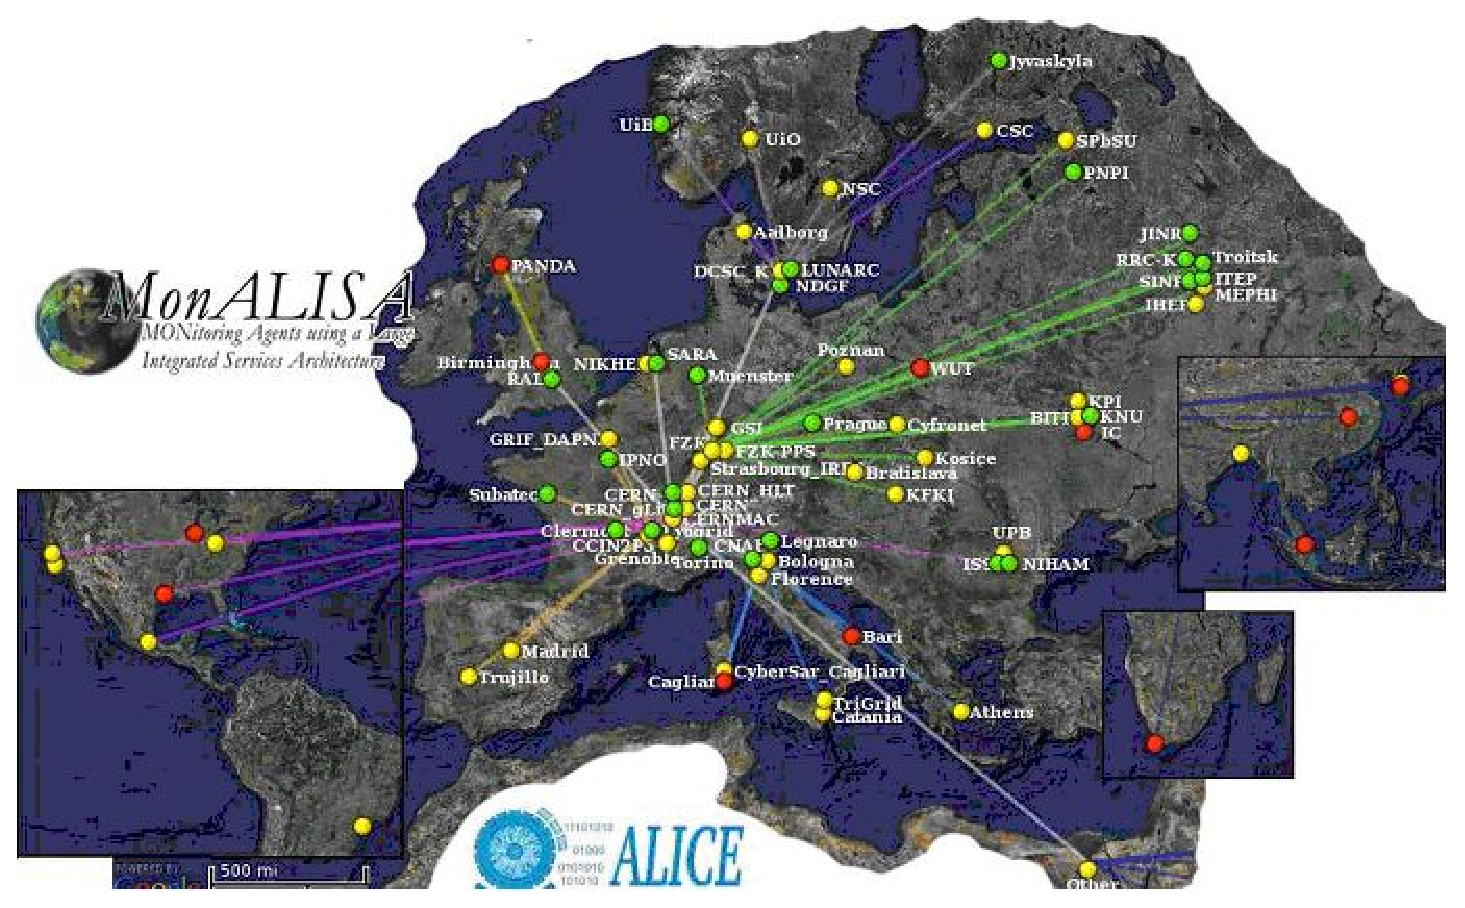
\includegraphics[width=13cm]{fig14.eps} %    ** if .eps don't need extension
\caption{ALICE sites}\label{fig14}
\end{figure}


\subsection{Concluding remarks}
%
The concept of the ALICE computing model was officially proposed in
2005. Since then, it has been used for massive Monte Carlo event
productions, for end-user analysis and for the raw data management
and processing. The strategy has been validated under heavy load
during a series of Data Challenges and during the real data taking
in 2010/2011. The model provides the required Grid functionality via
a combination of the common Grid services offered on the WLCG
resources and the ALICE-specific services from AliEn. Today's
computing environments are anything but static. Fast development in
Information Technologies, commodity hardware (hardware being
constantly replaced and operating systems upgraded), Grid software
and networking technologies inevitably boosted also further
development of the ALICE computing model. One of the main effects is
a transformation of the model from the strictly hierarchical
Tier-like structure to a more loose scenario, a ``cloud-like''
solution.

%%%%%%%%%%%%%%%%%%%% section 5 %%%%%%%%%%%%%%%%%%%%%%%%%%%%%%%%%%%%%%%%%%%%%%%%%%%%%%

\section{AliEn}

AliEn [26] is a set of middleware tools and services which represents
an implementation of the ALICE distributed computing environment
integrated in the WLCG environment. AliEn has been under a constant
development by ALICE since about 2001 and was deployed over the
ALICE Grid infrastructure right from the start. One of the important
features is the set of interfaces to other Grid implementations like
gLite [53], ARC [54] and OSG [15].

AliEn was initially developed as a distributed production
environment for the simulation, reconstruction, and analysis of
Physics data. Since it was put in the production in 2001, ALICE has
been using AliEn before the start of  the real data taking for
distributed production cycles of Monte-Carlo simulated raw data,
including subsequent reconstruction and analysis, during the regular
Physics Data Challenges. Since 2005, AliEn has been used also for
end-user analysis.  Since December 2007, when the ALICE detector
started operation taking cosmic data, AliEn has been used also for
management of the raw data.  Since the LHC startup in 2009, millions
of jobs have been successfully processed using the AliEn services
and tools.

AliEn developers provided the users with a client/interface - ``alien
shel'' [55] and a set of plugins designed for the end users' job
submission and handling. These tools together with the tools
provided by the ALICE Grid monitoring framework MonALISA [40] hide
the complexity and heterogenity of the underlying Grid services from
the end-user while facing the rapid development of the Grid
technologies.

AliEn is a lightweight Open Source Grid framework built around Open
Source components using the combination of standard network
protocols, a Web Service and Distributed Agent Model [26]. The basic
AliEn components include:
%
\begin{itemize}
\item AliEn File Catalogue with metadata capabilities
\item  Data management tools for data transfers and storage
\item Authentication, authorization and auditing services
\item Workload management system
\item Storage and computing elements
\item Information services
\item Site services
\item Command line interface - the AliEn shell aliensh
\item ROOT interface
\item Grid and job monitoring
\item Interfaces to other Grids
\end{itemize}

AliEn was primarily developed by ALICE, however it was adopted also
by a couple of other Virtual Organizations like e.g. PANDA [56].

\subsection{File Catalogue (FC)}
%
The File Catalogue is one of the key components of the AliEn suite.
It provides a hierarchical structure (like a UNIX File system) and
is designed to allow each directory node in the hierarchy to be
supported by different database engines, running on different hosts.
This building on top of several databases allows to add another
database to expand the catalogue namespace and assures scalability
of the system and allow growth of the catalogue as the files
accumulate over the years.

Unlike real file systems, the FC does not own the files; it is a
metadata catalogue on the Logical File Names (LFN) and only keeps an
association/mapping between the LFNs and (possibly multiple)
Physical File Names (PFN) of real files on a storage system. PFNs
describe the physical location of the files and include the access
protocol (rfio, xrootd), the name of the AliEn Storage Element and
the path to the local file. The system supports file replication and
caching.

The FC provides also a mapping between the LFNs and Globally Unique
Identifiers (GUID). The labeling of each file with the GUID allows
for the asynchronous caching. The write-once strategy combined with
GUID labeling guarantees the identity of files with the same GUID
label in different caches. It is possible to automatically construct
PFNs : to store only the GUID and Storage Index and the Storage
Element builds the PFN from the GUID. There are two independent
catalogues: LFN->GUID and GUID->PFN. A schema of the AliEn FC is
shown in Figure~\ref{fig15}.

%fig15
\begin{figure}[htb] % h-here, t-top, b-bottom
\centering
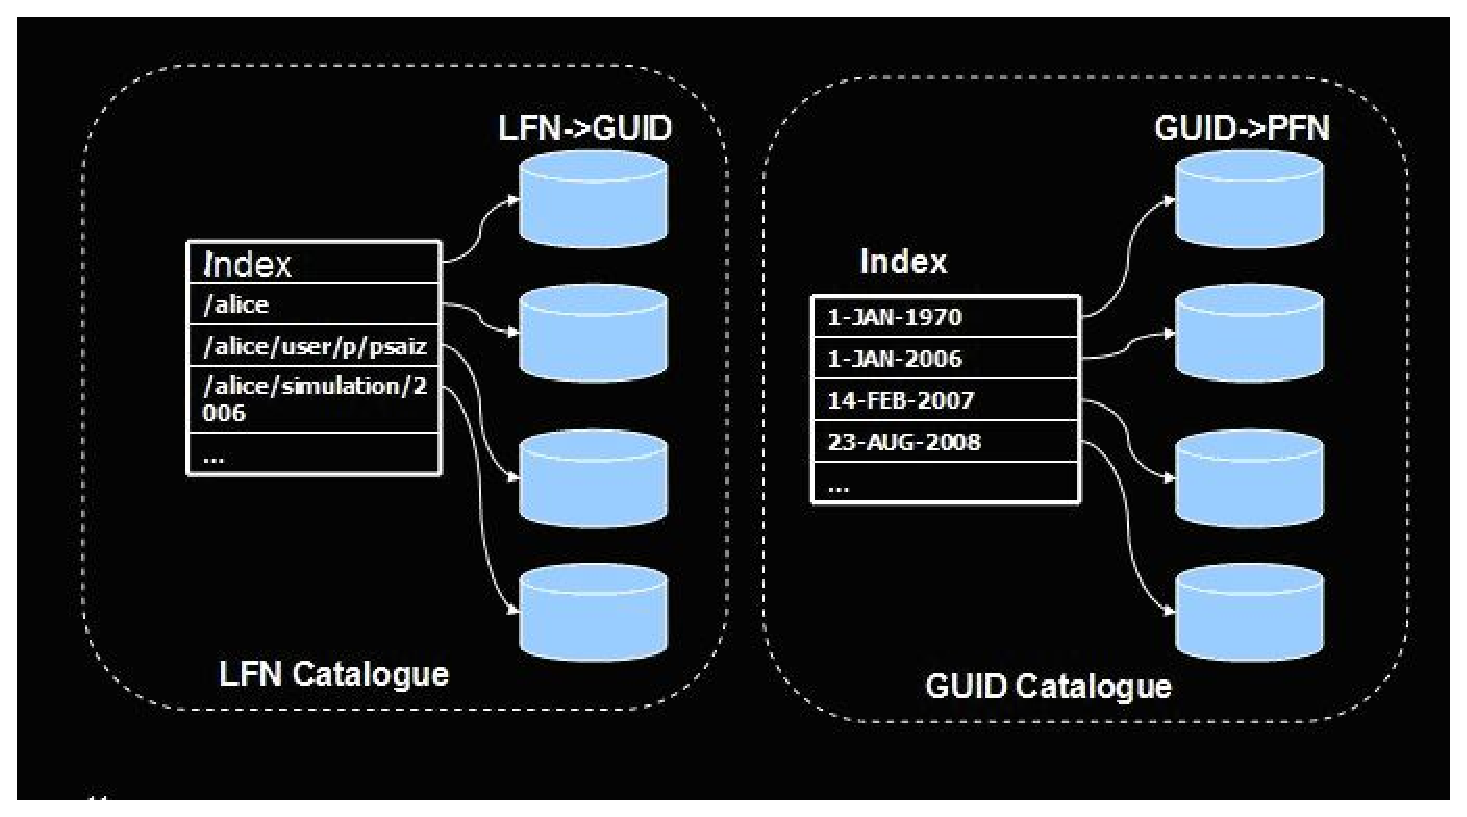
\includegraphics[width=13cm]{fig15.eps} %    ** if .eps don't need extension
\caption{AliEn File Catalogue}\label{fig15}
\end{figure}


\subsection{Authentication and Authorization}
%
The authentication uses the Grid Access Service (GAS) [57] which is
functioning as an ad-hoc user portal. Before connecting to GAS, a
user creates a proxy certificate and stores it in the myproxy server
and submits a session request. In addition to myproxy service, the
Virtual Organization Membership Service [58] is also used. The system
is able to take into account user roles when creating the GAS
interface.

\subsection{Workload Management System}
%
AliEn's Workload Management System (WMS) is based on the pull
architecture and is a set of central components (Task Queue, Job
Optimizer, Job Broker) and site components (Computing Element (CE),
Cluster Monitor, MonALISA, Package Manager). The pull architecture
has an advantage with respect to the push one: WMS does not have to
know actual status of all resources, which is crucial for large
flexible Grids. When the push architecture is used, WMS must get,
keep and analyze a huge amount of status data just to assign a job,
which becomes difficult in the expanding grid environment. In the
pull architecture, local agents (pilot status-checking test jobs)
running at individual sites ask for  real jobs after having checked
the local hardware and software conditions and found them
appropriate for the processing of the job. Thus the WMS only deals
with the requests of local pilot jobs, so called Job Agents (JA), to
assign appropriate real jobs. The descriptions of jobs in the form
of ClassAds are managed by the central Task Queue.

At each site, there are running AliEn services CE, ClusterMonitor,
Package Manager (PackMan) and a MonALISA client. The AliEn CE
automatically generates and submits to the local WLCG CE, or
eventually to an appropriate external Resource Broker or WMS, the
local Job Agents. The ClusterMonitor manages the connections between
the site and central services, so there is only one connection from
each site. The AliEn WMS can be integrated with WLCG or other Grid
systems WMS and the job management is organized by a collaboration
of both systems. Sites using AliEn are as a rule running some
services of the gLite, ARC or OSG, like e.g. CREAM-CE (see section
3).  The AliEn CE is in this case combined with the CREAM-CE in the
job submission machinery. Schemas of the job submission procedure in
AliEn are shown in Figures~\ref{fig16} and~\ref{fig17}.

%fig16
\begin{figure}[htb] % h-here, t-top, b-bottom
\centering
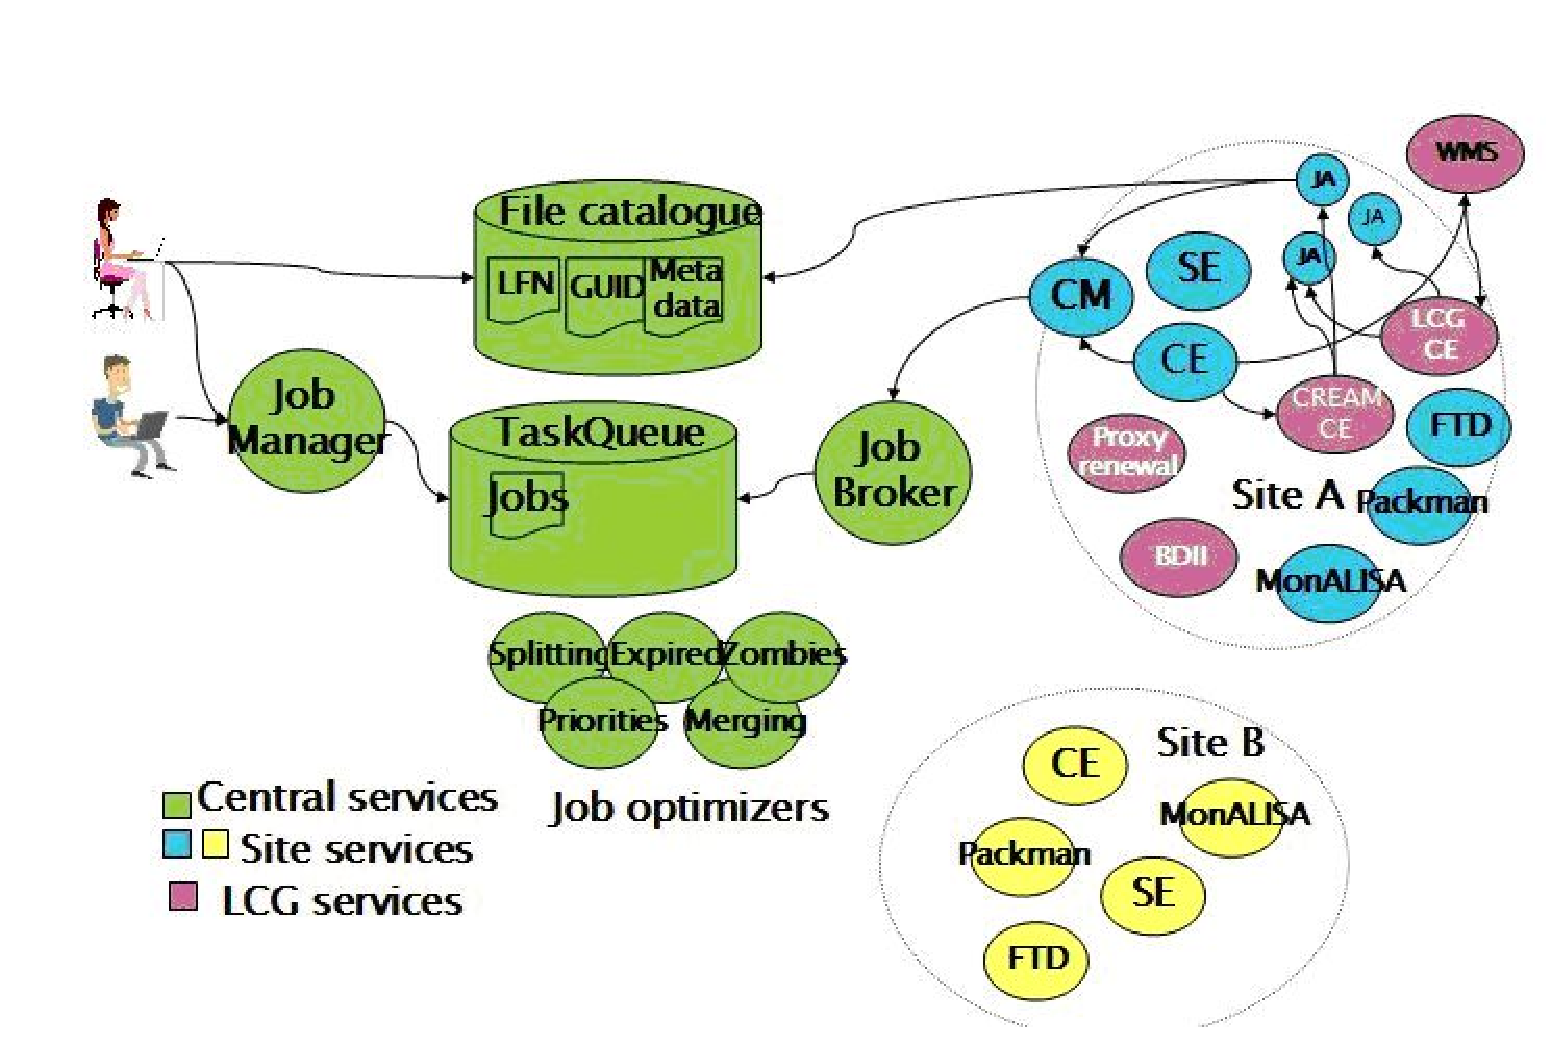
\includegraphics[width=13cm]{fig16.eps} %    ** if .eps don't need extension
\caption{AliEn + WLCG services}\label{fig16}
\end{figure}



%fig17
\begin{figure}[htb] % h-here, t-top, b-bottom
\centering
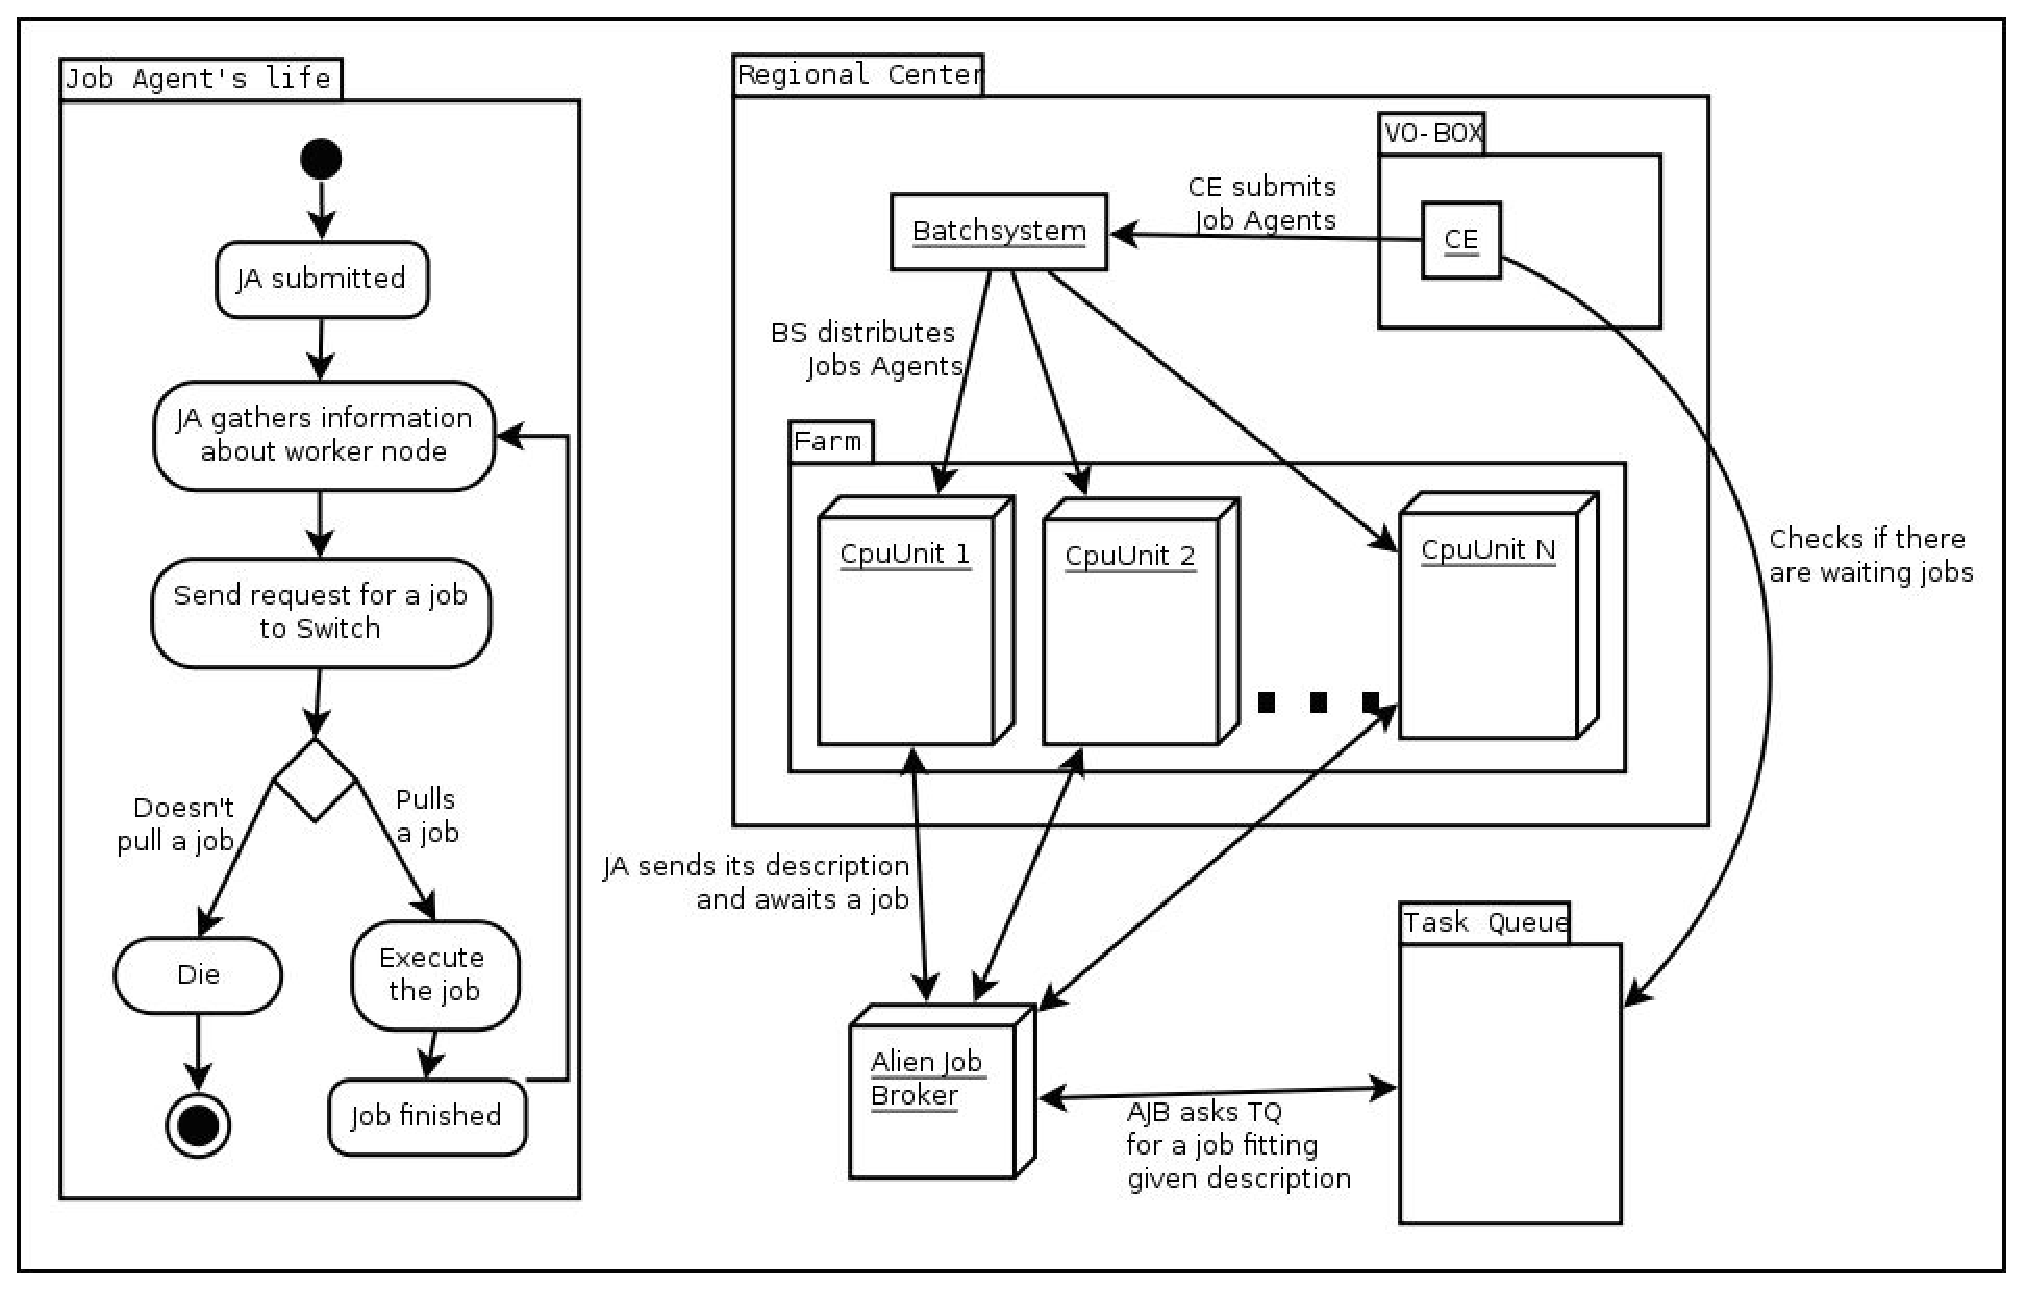
\includegraphics[width=13cm]{fig17.eps} %    ** if .eps don't need extension
\caption{The Job Agent model in AliEn}\label{fig17}
\end{figure}



\subsection{Jobs}
%
When a job is submitted by a user, its description in the form of a
ClassAd is kept in the central TQ (handling also priorities and
quotas) where it waits for a suitable Job Agent for execution.  The
requirements of all jobs waiting in the central TQ are checked by
the central Job Optimizer. It can change some requirements, or
suggest data transfers so it would be more likely that some Job
Agent picks up the job.

After it has been submitted, a job gets through several stages, see
[59].  The information about running processes is kept also in the
AliEn FC. Each job is given a unique id and a corresponding
directory where it can register temporary files, standard input and
output as well as all job products. So while the information on job
submission and status is centralized, the decisions concerning the
actual submission is decentralized: sites decide which job to
"pull". The JAs provide a job-wrapper, a standard environment
allowing a virtualization of resources. The whole job submission and
processing chain is extensively monitored so a user can any time get
the information on the status of his/her jobs.

\subsection{Site services}
%
As mentioned efore, at each ALICE site are
running AliEn services CE, ClusterMonitor, PackMan and MonALISA.
These services are running on a dedicated machine, so called VOBOX
described in section 3.

The AliEn site CE is usually associated with the local batch system.
It is periodically submitting testing pilot jobs (Job Agents)  to
the local WLCG CE or an appropriate external Resource Broker or WMS.
The role of the Job Agents is to verify the local hardware and
software capacities at the site. After the usual matchmaking
procedure, the JA is sent, through the site CE, into the local batch
queue and then to a local Worker Node (WN). After its startup, the
JA performs its task and in the case of a positive checkup, the JA
requests a "real" job from the central Task Queue via the AliEn Job
Broker, or dies otherwise.

The PackMan automates the process of installation, upgrades,
configuration and removal of the ALICE software packages from the
shared software area on the site. It also advertises known/installed
packages. The packages are installed on demand, when requested by a
Job Agent running on a Worker Node or during the central software
deployment over the Grid sites. If a package is not already
installed the PackMan would install it along with its dependencies
and return a string with commands that client has to execute to
configure the package and all its dependencies. The PackMan manages
the local disk cache and cleans it, when it needs more space to
install newer packages.

The Cluster Monitor handles communication with the AliEn Job Broker
and gives configuration to JAs.  It gets ``heartbeats'' from the JAs.
If it gets no heartbeats from a JA, the existing job will get into
the ZOMBIE status (after 1.5 hours) and then it will expire (after 3 hours).

The site services include also a MonALISA client and File Transfer
Daemon (FTD), described in the following.

\subsection{Monitoring}
%
Since the AliEn Workload Management does not
depend directly on sophisticated monitoring, no special monitoring
tools were developed in AliEn. As the monitoring solution, ALICE has
adopted and further developed the Java-based MonALISA [40] framework
mentioned already in the previous section. The MonALISA system is
designed as an ensemble of autonomous multithreaded, self-describing
agent-based subsystems which are registered as dynamic services, and
together can collect and process large amounts of information [40].

The collected monitoring information is published via Web Service
for use by AliEn Optimizers or for visualization purposes. An
extension of the network simulation code which is a part of MonALISA
can provide a tool for optimization and understanding of the
performance of the AliEn Grid system.

\subsection{File Transfer}
%
This service provides the scheduled file transfer
functionality and is running at the Storage Elements contained in
the ALICE distributed storage cluster. The File Transfer Daemons
(FTD) perform file transfers between sites on user's behalf using a
suitable external transfer protocol (like e.g. bbFTP or GridFTP).
File transfers are requested and scheduled in exactly the same way
as production jobs, this time under the control of the File Transfer
Broker.

\subsection{Storage}
%
Experience with the performance of different types of storage
managers shows that the most advanced storage solution is the native
XRootD [33] manager described in section 3. It has been demonstrated
that with all other parameters being equal (protocol access speed
and security) the native XRootD storage clusters exhibit
substantially higher stability and availability. The ALICE
distributed system of native XRootD clusters is orchestrated by the
global redirector which allows interacting with the complete storage
pool as a unique storage.  All storages are on WAN (Wide Area
Network).

\subsection{AliEn Shell - aliensh}
%
To complete the brief description of AliEn, we mention the client
called AliEn shell. It provides a UNIX-shell-like environment with
an extensive set of commands which can be used to access AliEn Grid
computing resources and the AliEn virtual file system.  There are
three categories of commands: informative and convenience commands,
File Catalogue and Data Management commands and TaskQueue/Job
Management commands. The AliEn shell has been created about 4 years
ago and become a popular tool among the users for job handling and
monitoring.

\subsection{Concluding remarks}
%
AliEn is a high-level middleware adopted by
the ALICE experiment, which has been used and validated in massive
Monte Carlo events production since 2001, in end-user analysis since
2005 and during the real data management and processing since 2007.
Its capabilities comply with the requirements of the ALICE computing
model. In addition to modules needed to build a fully functional
Grid, AliEn provides interfaces to other Grid implementations
enabling the true Grid interoperability. The AliEn development will
be ongoing in the coming years following the architectural path
chosen at the start and more modules and functionalities are
envisaged to be delivered.

The Grid (AliEn/gLite/other) services are many and quite complex.
Nonetheless, they are working together, allowing to manage thousands
of CPUs and PBs of various storage types. The ALICE choice of single
Grid Catalogue, single Task Queue with internal prioritization and a
single storage access protocol (xrootd) has been beneficial from
user and Grid management viewpoint.



%%%%%%%%%%%%%%%%%%%% section 6 %%%%%%%%%%%%%%%%%%%%%%%%%%%%%%%%%%%%%%%%%%%%%%%%%%%%%%

\section{WLCG and ALICE performance during the 2010/2011 LHC data
taking}

In this section, we will discuss the experience and performance of
the WLCG in general and the ALICE Grid project in particular during
the real LHC data taking both during the proton and the lead ion
beam periods.

\subsection{LHC performance}
%
The LHC delivered the first pp collisions in the end of 2009, but
the stable operations startup was in March 2010. Since then, the
machine has been working amazingly well compared to other related
facilities. Already in 2009, the machine beaten the world record in
the beam energy and other records have followed. In 2010, the
delivered integrated luminosity was 18.1 pb${}^{-1}$ and already
during the first months of operation in 2011, the delivered
luminosity was 265 pb${}^{-1}$. This is about a quarter of the
complete target luminosity for 2010 and 2011 [60], which is supposed
to be sufficient to get the answer concerning the existence of the
Higgs boson. Also, as mentioned in section 1, the machine has beaten
the records concerning the stored energy and also the beam
intensity.

The target number of bunches per a beam of protons stated for 2011
was reached already in the middle of the year: 1380 bunches. The
final target luminosity of $10^{34}\ $cm${}^{-2}$s${}^{-1}$ is being
approached rapidly, at present it is about
$10^{33}\ $cm${}^{-2}$s${}^{-1}$ [61].


\subsection{WLCG performance}
%
The performance of the data handling by the WLCG has also been
surprisingly good. This wrapped up several years to the LHC startup,
when the WLCG and the experiments themselves were regularly
performing a number of stress-tests of their distributed computing
infrastructure and were gradually upgrading the systems using new
technologies. As a result, when the data started to flow from the
detectors, the performance of the distributed data handling
machinery was quite astounding.  All aspects of the Grid have really
worked for the LHC and have enabled the delivery of Physics results
incredibly quickly.

During 2010, 15 PetaBytes of data were written to tapes at the CERN
Tier-0 reaching the level expected from the original estimates for
the fully-tuned LHC operations, a nominal data taking year. As
mentioned in section 2, in average 2 PB of data per a month were
written to tapes at Tier-0 with the exception of the heavy ions
period when this number got about doubled and a world record was
reached with 225~TB written to tapes within one day [17], see
Figure~\ref{fig18}. The CERN Tier-0 moved altogether above 1~PB of
data per day [17].

%fig18
\begin{figure}[htb] % h-here, t-top, b-bottom
\centering
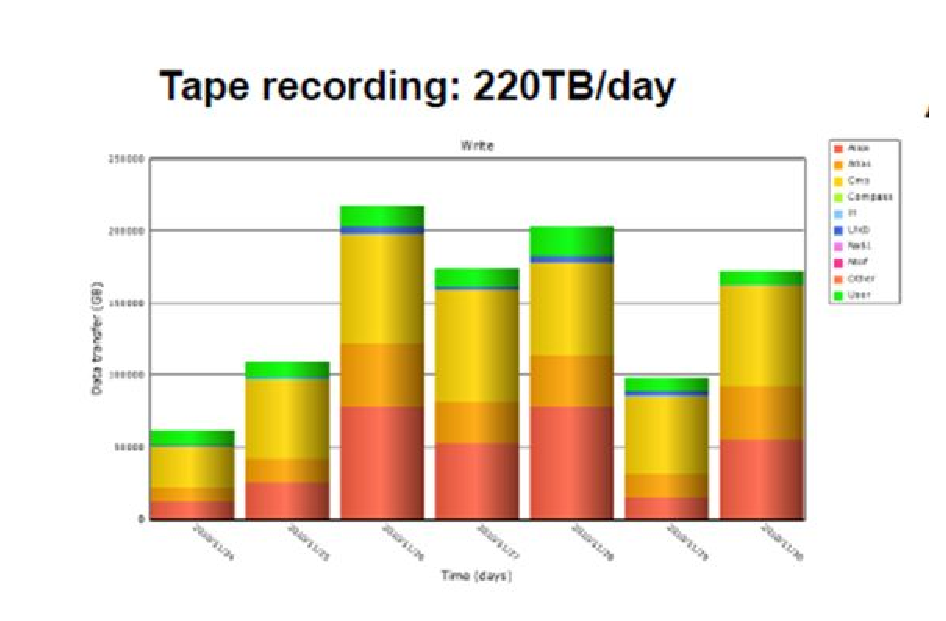
\includegraphics[width=13cm]{fig18.eps} %    ** if .eps don't need extension
\caption{A record in data tape recording: over
220~TB/day}\label{fig18}
\end{figure}


As mentioned in section 2, the mass storage system at the CERN
Tier-0 supported data rates at an average over the year of ~
2.5~GB/s IN with peaks up to 11~GB/s, and data was served at an
average rate of $\sim 7$~GB/s with peaks up to 25~GB/s.

The data processing went on without basic show-stoppers. The
workload management system was able to get about 1 million of jobs
running per day, see Figure~\ref{fig19}, and this load is
gradually going up. This translates into significant amounts of
computer time. Towards the end of 2010 there was a situation when
all of the available job slots at Tier-1s and Tier-2s were often
fully occupied. This has been showing up also during 2011, so the
WLCG collaboration has already now fully used all the available
computing resources. During 2010, the WLCG delivered about
100~CPU-millennia [17].

%fig19
\begin{figure}[htb] % h-here, t-top, b-bottom
\centering
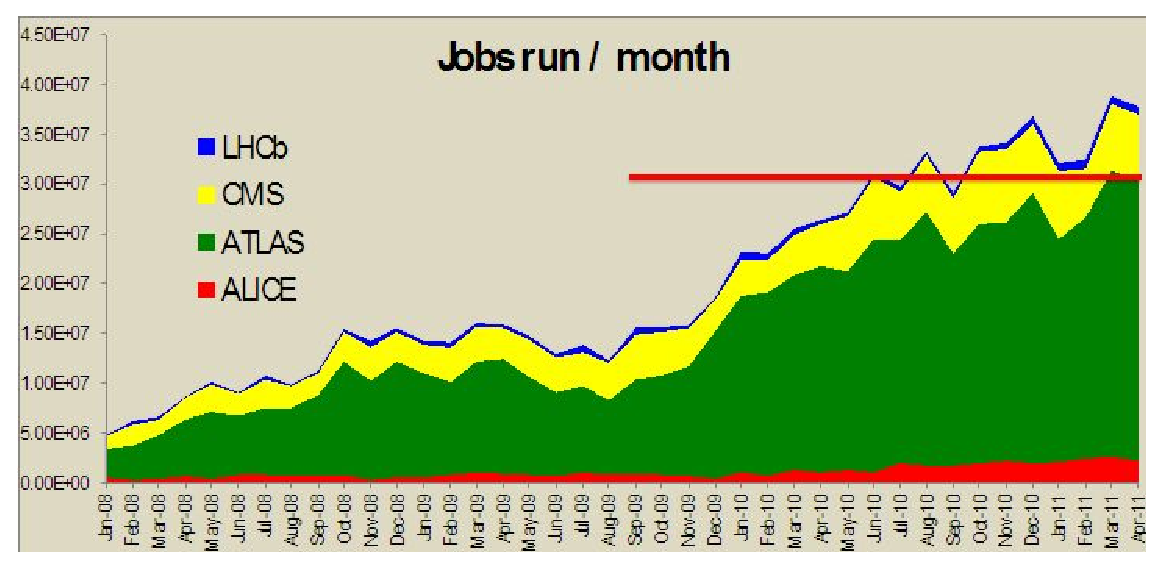
\includegraphics[width=13cm]{fig19.eps} %    ** if .eps don't need extension
\caption{WLCG job profile}\label{fig19}
\end{figure}



As also briefly mentioned in section 2, the WLCG was very successful
concerning the number of individuals really using the grid to
perform their analysis. At the start of the project, there was a
concern that end users will be discouraged from using the grid due
to complexity of its structure and services. But thanks to the
effort of the WLCG and experiments themselves a reasonably simple
access interfaces were developed and the number of end users reached
up to 800 in the large experiments.

The distribution of the delivered CPU power between sites has been
basically according to the original design, but the Tier-2s provided
more than the expected 40\%: it was in fact 50\% or more of the
overall delivery, see section 2. Member countries pledged different
amounts of resources according to their capacities and have been
delivering accordingly.  So the concept of collaborative Grid
resource sharing really works and enables institutes worldwide to
share data, and provide resources to the common goals of the
collaboration.

\subsubsection{Network performance}
%
The key basis for building up a distributed system is the data
transfer infrastructure. The network which the WLCG operates today
is much in advance of what was anticipated in the time of writing
the WLCG TDR. The OPN [18], see also section 2, started as dedicated
fiber links from CERN to each of the Tier-1s with the throughput 10
Gbit/s. Today, there is a full redundancy in this network with the
original links doubled and with back-up links between Tier-1s
themselves. The OPN is a complicated system with many different
layers of hardware and software and getting it into the current
shape was a difficult task, which evidently paid-off.

The original concerns about the possible network unreliability and
insufficiency were not realized. The network infrastructure relying
on the OPN and the complementary GEANT, US-LHCNet and all the R\&E
national network infrastructures, extensively monitored and
continuously checked with the test transfer jobs, has never been a
problem in the data transfer except for occasional glitches. The
originally estimated sustained transfer rate of 1.3~GB/s from Tier-0
to Tier-1s was reached without problems and exceeded and reached up
to 5~GB/s. Within the OPN, a peak of 70~Gb/s was supported without
any problem during a re-processing campaign of one of the LHC
experiments, see Figure~\ref{fig20}.

%fig20
\begin{figure}[htb] % h-here, t-top, b-bottom
\centering
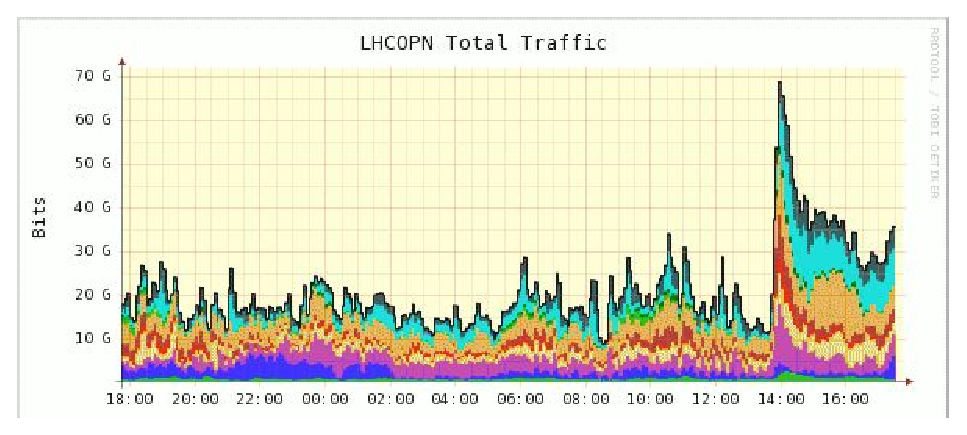
\includegraphics[width=13cm]{fig20.eps} %    ** if .eps don't need extension
\caption{WLCG OPN traffic in 2010 with a peak of 70
Gbit/s}\label{fig20}
\end{figure}



\subsubsection{Concluding remarks - WLCG}
%
The experience from the first year and a half of the LHC data taking
implies that the WLCG has built a truly working grid infrastructure.
The LHC experiments have their own distributed models and have used
the WLCG infrastructure to deliver Physics results within weeks
after the data recording which has never been achieved before. The
fact that a significant numbers of people are doing analysis on the
Grid, that all the resources are being used up to the limits and the
scientific papers are produced with an unprecedented speed is
proving an evident success of the WLCG mission.


\subsection{ALICE performance}
%
To conclude this section, we will briefly summarize the experience
and performance of the ALICE experiment. ALICE started extremely
successfully the processing of the LHC data in 2009: the data
collected during the first collisions delivered by the LHC on
November 23rd (2009) got processed and analyzed so fast that within
one week the article with the results from the first collisions was
accepted for publication as the first ever scientific paper with the
Physics results from the LHC collisions [62].

\subsubsection{Jobs}
%
During the data taking in 2010, ALICE collected 2.3~PB of raw data,
which represented about 1.2 million of files with the average file
size of 1.9~GB. The data processing chain has been performing
without basic problems.  The Monte Carlo simulation jobs together
with the raw data reconstruction and organized analysis (altogether
the organized production) represented almost 7 millions of
successfully completed jobs, which translates into 0.3 jobs/second.
The chaotic (end user) analysis made for 9 millions of successfully
completed jobs, which represents 0.4 jobs/s, consuming approximately
10\% of the total ALICE CPU resources (the chaotic analysis jobs are
in general shorter than the organized processing jobs).  In total,
there were almost 16 millions of successfully done jobs, which
translates to ~1 job/s and 90 thousands jobs/day. The complimentary
number of jobs which started running on the Grid but finished with
an error was in excess of this.

The running jobs profile got in peaks to 30 thousands of
concurrently running jobs (see Figure~\ref{fig21}) with more than
50\% of the CPU resources delivered by the Tier-2 centers. About
60\% of the total number of jobs represented the end user analysis
(see Figure~\ref{fig22}). In general, the user analysis already in
2010 was a resounding success, with almost 380 people actively using
the Grid. Since the chaotic analysis brings sometimes problems
concerning not completely perfect code resulting, e.g., in a high
memory consumption (cf. section 4), ALICE was running a mixture of
the organized production and end user jobs at all its sites, and
this scenario was working well.

%fig21
\begin{figure}[htb] % h-here, t-top, b-bottom
\centering
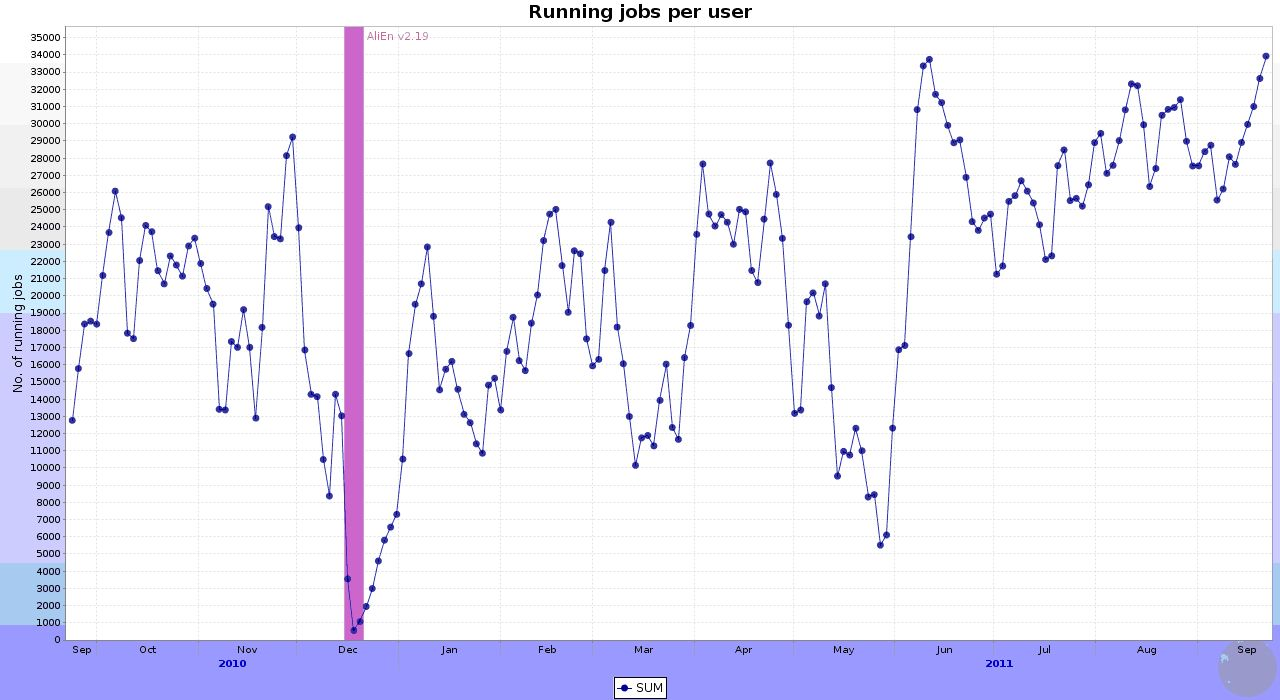
\includegraphics[width=13cm]{fig21.eps} %    ** if .eps don't need extension
\caption{ALICE running jobs profile 2010/2011}\label{fig21}
\end{figure}


%fig22
\begin{figure}[htb] % h-here, t-top, b-bottom
\centering
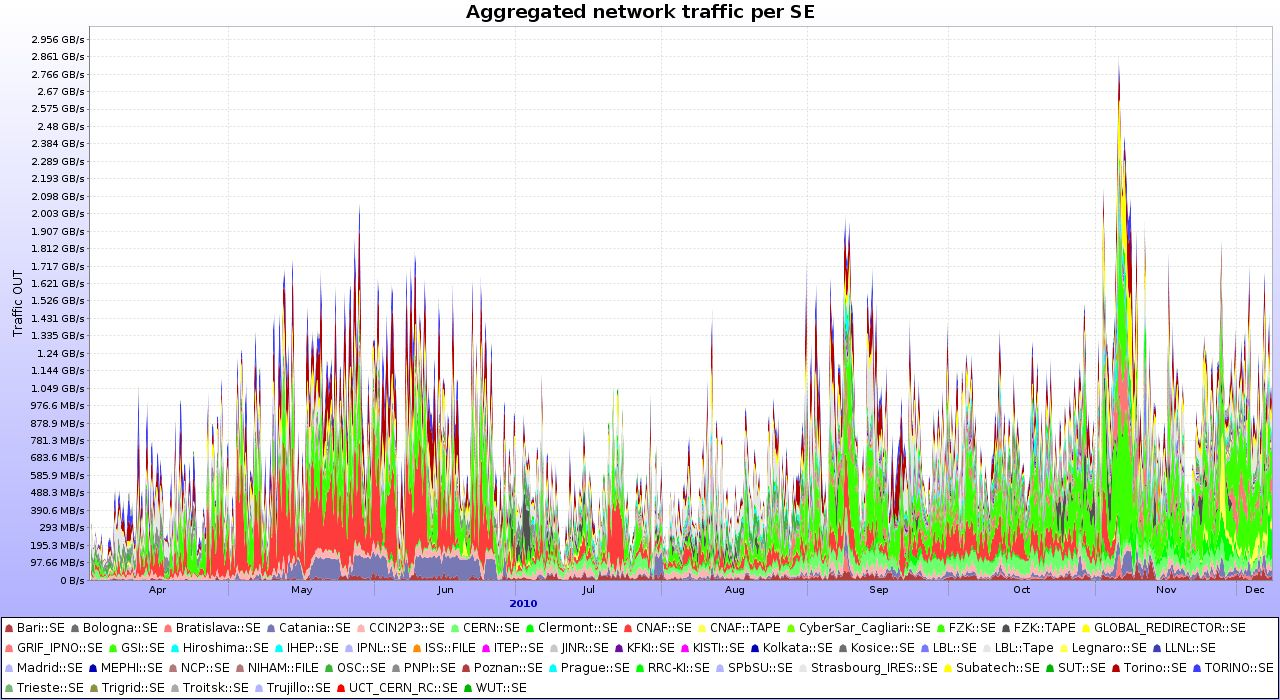
\includegraphics[width=13cm]{fig22.eps} %    ** if .eps don't need extension
\caption{Network traffic OUT by analysis jobs - 2010}\label{fig22}
\end{figure}



\subsubsection{Storage-2010}
%
The distributed storage system endured and was supporting an
enormous load. During 2010/2011, 25.15 PB of data (raw, ESDs, AODs,
Monte Carlo  productions) was written to xrootd Storage Elements
with the speed maximum of 621.1 MB/s. 59.97 PB  of data was read
from the xrootd Storage Elements, with the speed maximum of 1.285
GB/s, see Figure~\ref{fig23}.

%fig23
\begin{figure}[htb] % h-here, t-top, b-bottom
\centering
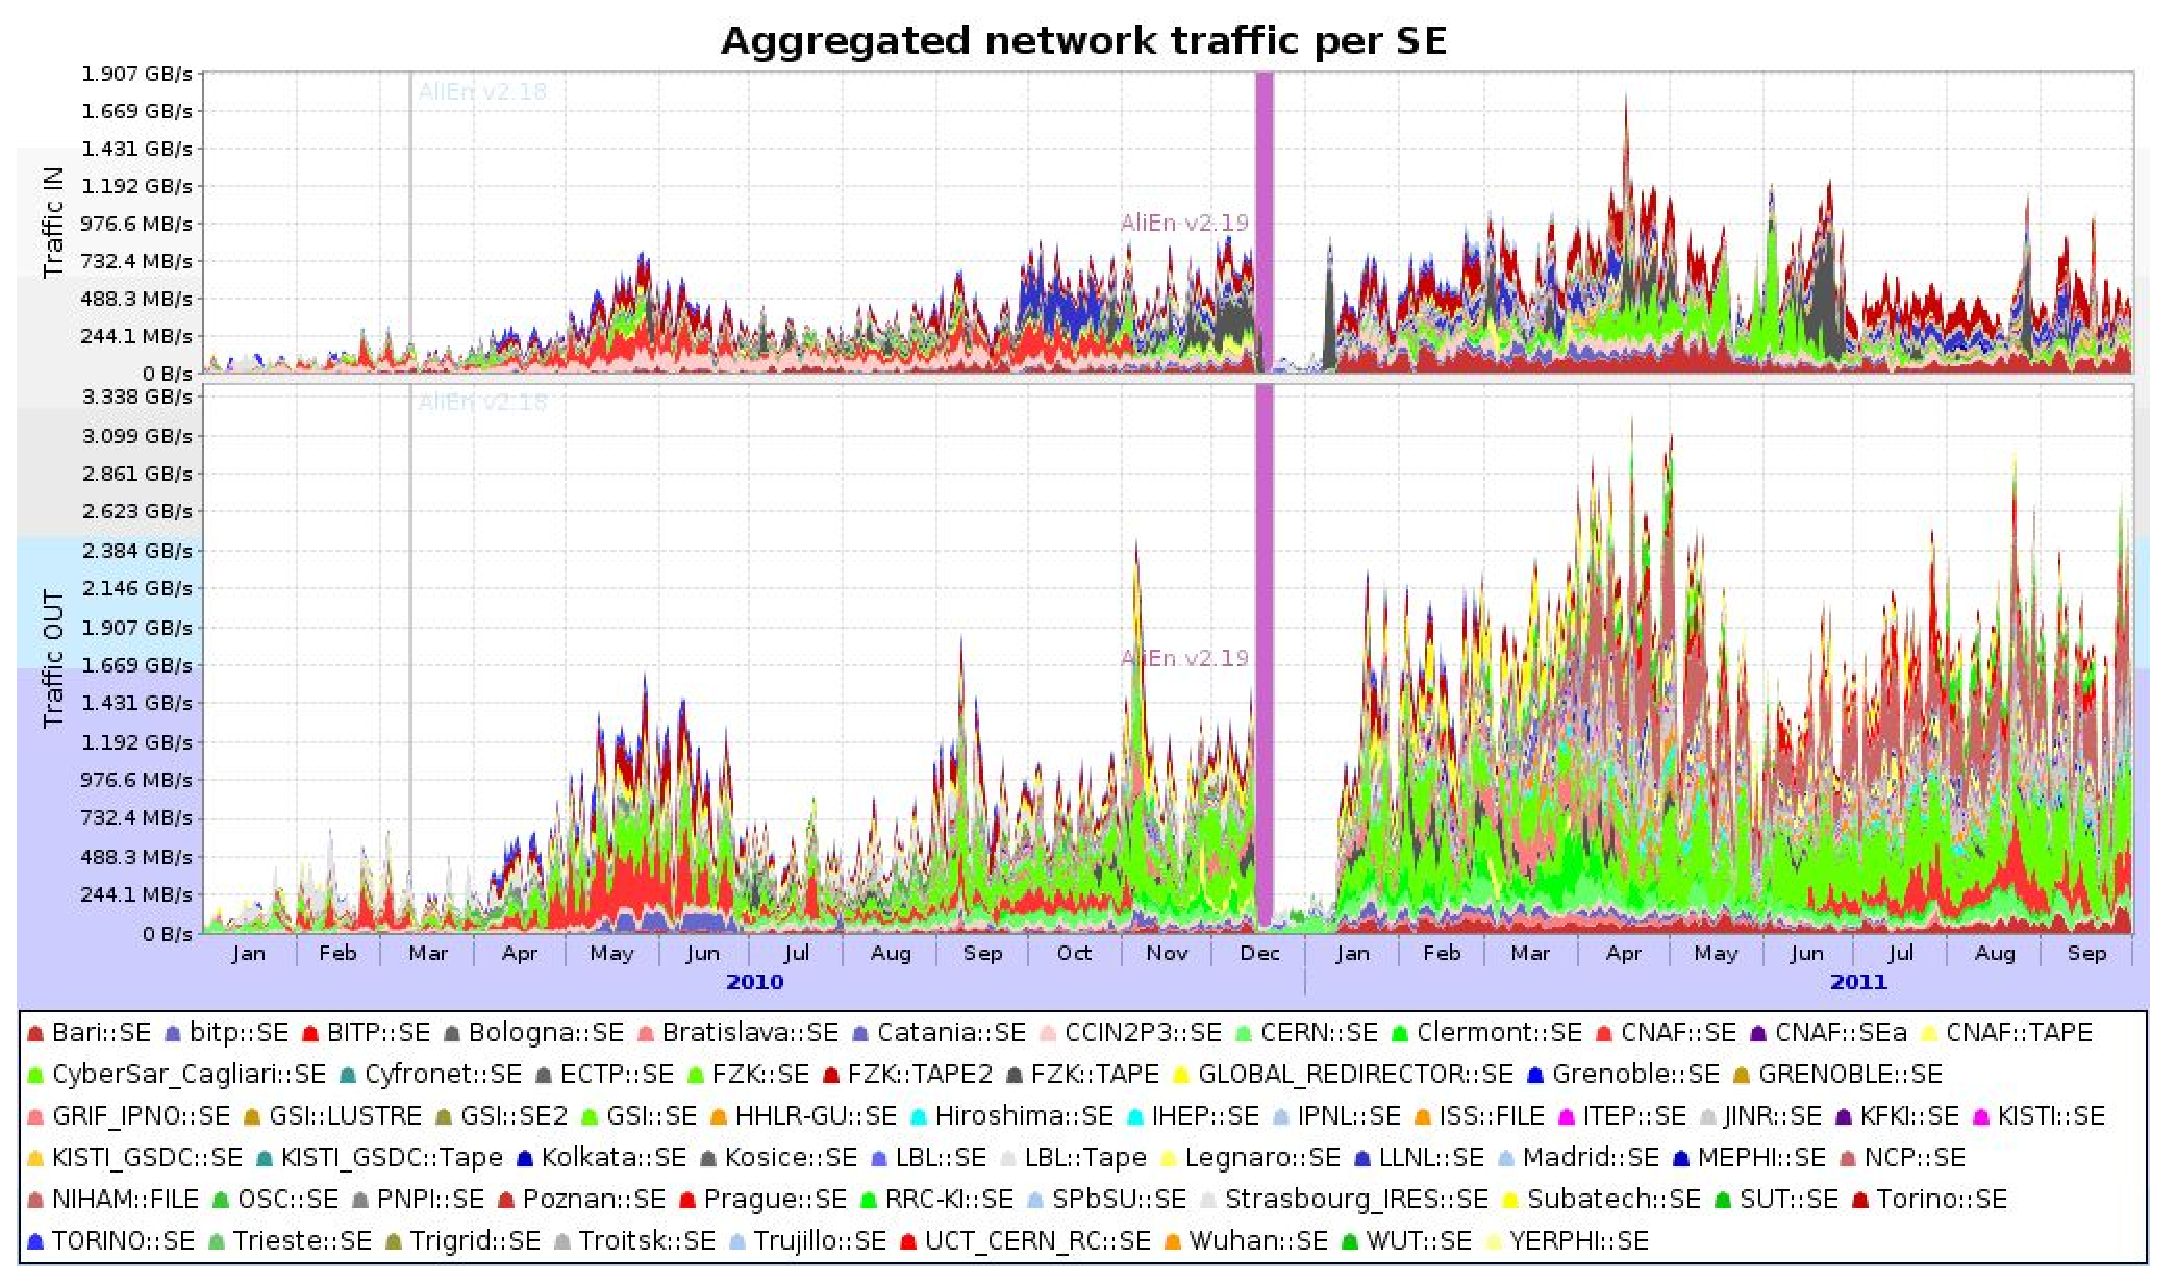
\includegraphics[width=13cm]{fig23.eps} %    ** if .eps don't need extension
\caption{Total network traffic at the ALICE Storage Elements -
2010/2011}\label{fig23}
\end{figure}


\subsubsection{Data taking 2011}
%
Constantly upgrading and extending its hardware resources and
updating the grid software, ALICE continued a successful LHC data
handling campaign in 2011. By September, the total volume of the
collected raw data was almost 1.7~PB with the first reconstruction
pass completed. 2011 was marked by massive user analysis on the
Grid. In May, the most important conference in the Heavy Ion Physics
community, Quark Matter 2011 (QM2011) [63], took place and was
preceded by an enormous end user analysis campaign. In average, 6
thousands end-user jobs were running all the time, which represents
almost 30\% of the CPU resources officially dedicated to ALICE (The
number of running jobs is higher than that most of the time due to
use of opportunistic resources). During the week before the QM2011,
there was a peak with 20 thousands of concurrently running end-user
jobs, see Figures~\ref{fig23},\ref{fig24}. The number of active Grid
users reached 411.

%fig24
\begin{figure}[htb] % h-here, t-top, b-bottom
\centering
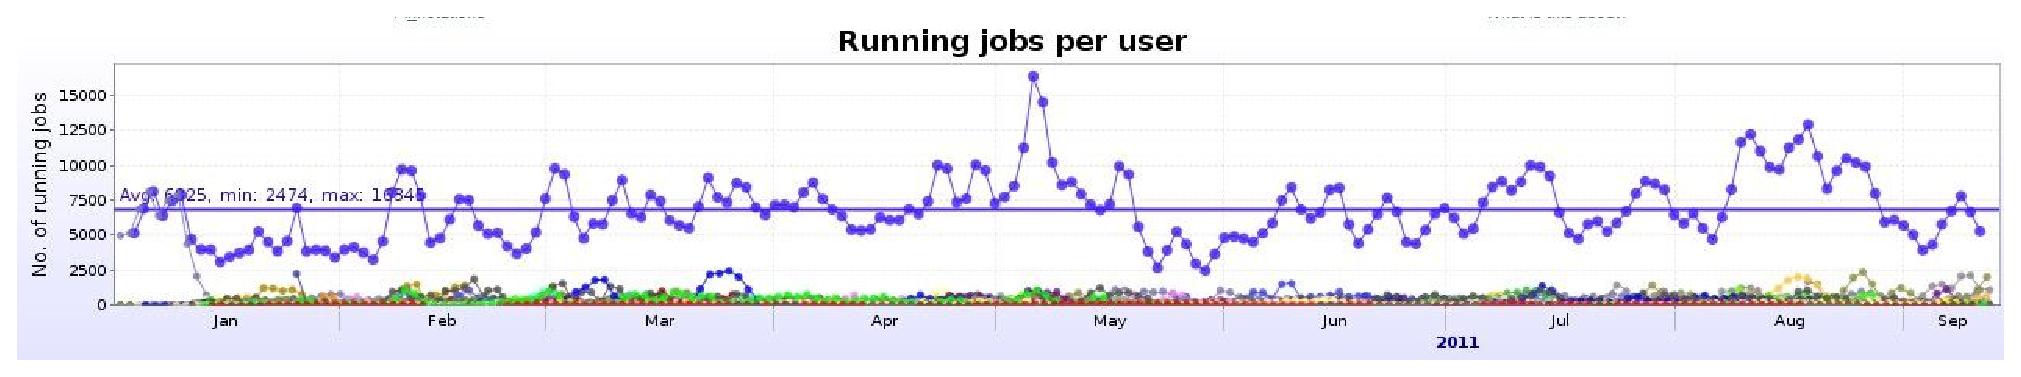
\includegraphics[width=13cm]{fig24.eps} %    ** if .eps don't need extension
\caption{End-user jobs profile - 2011}\label{fig24}
\end{figure}


In total, the ALICE sites were running in average 21 thousands of
jobs with peaks up to 35~thousands (Figure~\ref{fig21}). The
resources ratio remained 50\% delivered by Tier-0 and Tier-1s to
50\% delivered by Tier-2s. Altogether, 69 sites were active in the
operations. The sites' availability and operability kept very stable
throughout the year. The gLite (now EMI) middleware, see section 3,
is mature and only a few changes are necessary. To the end of the
year 2011, a new AliEn version with new central services and user
client is expected to be ready for deployment.

In the beginning of the 2011 campaign, there was a concern that the
storage would be saturated. In fact the storage infrastructure was
performing basically without problems supporting the enormous load
from the end-user analysis and was getting ready for the Pb-Pb
operations. The network situation, as was already mentioned for the
WLCG in general, has been excellent and allowed for the operation
scenario where the hierarchical tiered structure got blurred, the
sites of all levels were well interconnected and running a similar
mixture of jobs. As a result, the ALICE Grid in a sense has been
working as a cloud.

\subsection{Concluding remarks - ALICE}
%
In general, similar to the overall characteristics of the WLCG
performance also the ALICE operations and data handling campaigns
were notably successful right from the beginning of the LHC startup,
making the Grid infrastructure operational and supporting a fast
delivery of Physics results. By September 2011, ALICE has published
15 scientific papers with the results from the LHC collisions and
more is on the way. Two papers [64,65] were marked as ``Suggested
reading'' by the Physical Review Letters editors and the paper [65]
was selected for the ``Viewpoint in Physics'' by Physical Review
Letters.


%fig25
\begin{figure}[htb] % h-here, t-top, b-bottom
\centering
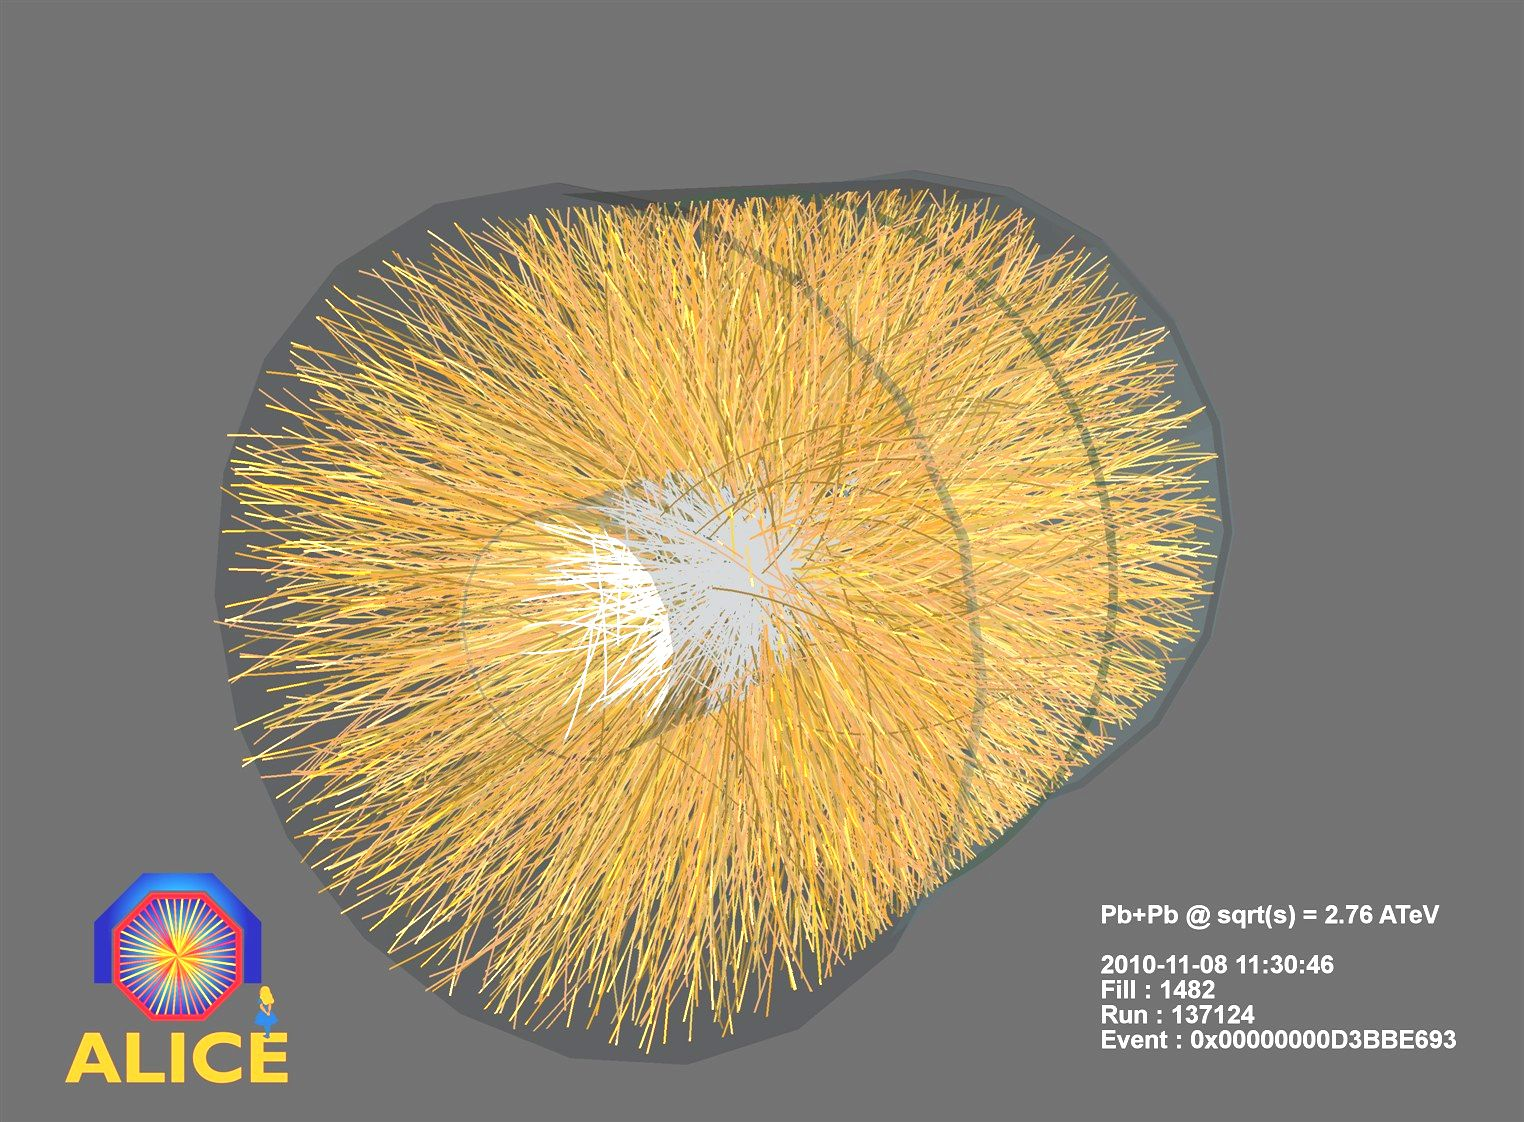
\includegraphics[width=13cm]{fig25.eps} %    ** if .eps don't need extension
\caption{Pb-Pb collision event recorded by ALICE}\label{fig25}
\end{figure}



The full list of the ALICE papers published during 2009-2011 can be
found on [66]. One of the Pb-Pb collision events recorded by ALICE is
shown on Figure~\ref{fig25}.


%%%%%%%%%%%%%%%%%%%% section 7 %%%%%%%%%%%%%%%%%%%%%%%%%%%%%%%%%%%%%%%%%%%%%%%%%%%%%%

\newpage

\section{Summary and Outlook}

This article is meant to be a short overview of the facts concerning
the Grid computing for HEP experiments, in particular for the
experiments at the CERN LHC. The experience gained during the LHC
operations in 2009-2011 has proven that for this community, the
existence of a well performing distributed computing
is necessary for the achievement and fast delivery of scientific
results. The existing WLCG infrastructure turned up to be able to
support the data production and processing thus fulfilling its
first-plan mission. It has been and will be continuously developing
into the future absorbing and giving rise to new technologies, like
the advances in networking, storage systems and inter-operability
between Grids and Clouds [67,68].

\subsection{Data management}
%
Managing the real data taking and processing in 2009-2011 provided
basic experience and a starting point for new developments. The
excellent performance of the network which was by far not
anticipated in the time of writing the WLCG (C)TDR shifted the
original concept of  computing models based on hierarchical
architecture to a more symmetrical mesh-like scenario. In original
design, the jobs are sent to sites holding the required data sets
and there are multiple copies of data spread over the system due to
anticipation that network will be unreliable or insufficient. It
turned out that some data sets were placed on sites and never
touched.

Based on the existing excellent network reliability and growing
throughput, the data models start to change along a dynamical
scenario. This includes sending data to a site just before a job
requires it, or reading files remotely over the network, use remote
(WAN) I/O to the running processes. Certainly, fetching over the
network one needed data file from a given data set which can contain
hundreds of files is more effective than a massive data sets
deployment and will spare storage resources and bring less network
load.

The evolution of the data management strategies is ongoing. It goes
towards caching of data rather than strict planned placement.  As
mentioned, the preferences go to fetching a file over the network
when a job needs it and to a kind of intelligent data pre-placement.
The remote access to data (either by caching on demand and/or by
remote file access) should be implemented.

\subsection{Network}
%
To improve the performance of the WLCG-operated network
infrastructure, the topology of LHC Open Network Environment (LHCONE [69])
is being developed and
built. This should be complementary to the existing OPN
infrastructure providing the inter-connectivity between Tier-2s and
Tier-1s and between Tier-2s themselves without putting an additional
load on the existing NREN infrastructures. As we learned during the
last years, the network is extremely important and better connected
countries do better [17].

\subsection{Resources}
%
During the 2010 data taking the available resources were sufficient
to cover the needs of experiments, but during 2011 the computing
slots as well as the storage capacities at sites started to be full.
Since the experience clearly shows that delivery of the Physics
results is limited by resources, the experiments are facing a
necessity of more efficient usage of existing resources. There are
task forces studying the possibility of using the next generations
computing and storage technologies. There is for instance a question
of using multicore processors which might go into the high
performance computing market while WLCG prefers usage of commodity
hardware.

\subsection{Operations}
%
Another important issue is sustainability and support
availability for the WLCG operations. The middleware used today for
the WLCG operations is considerably complex with many services
unnecessarily replicated in many places (like e.g. databases) mainly
due to original worries concerning network. The new conception is to
gradually search for more standard solutions instead of often highly
specialized middleware packages maintained and developed by WLCG.

\subsection{Clouds and Virtualization}
%
Among the new technologies, the Clouds is the right buzzword now and
the virtualization of resources comes along. The virtualization of
WLCG sites started prior to the first LHC collisions and has gone
quite far. It helps improving system management, provision of
services on demand, can make use of resources more effective and
efficient. Virtualization also enables to make use of industrial and
commercial solutions.

But, no matter what the current technologies advertise, the LHC
community will always use a Grid because the scientists need to
collaborate and share resources. No matter what technologies are
used underneath the  Grid, the collaborative sharing of resources
and the network of trust and all the security infrastructure
developed on the way of building the WLCG is of enormous value, not
only to WLCG community but to e-science in general. It allows people
to collaborate across the infrastructures.

%fig26
\begin{figure}[htb] % h-here, t-top, b-bottom
\centering
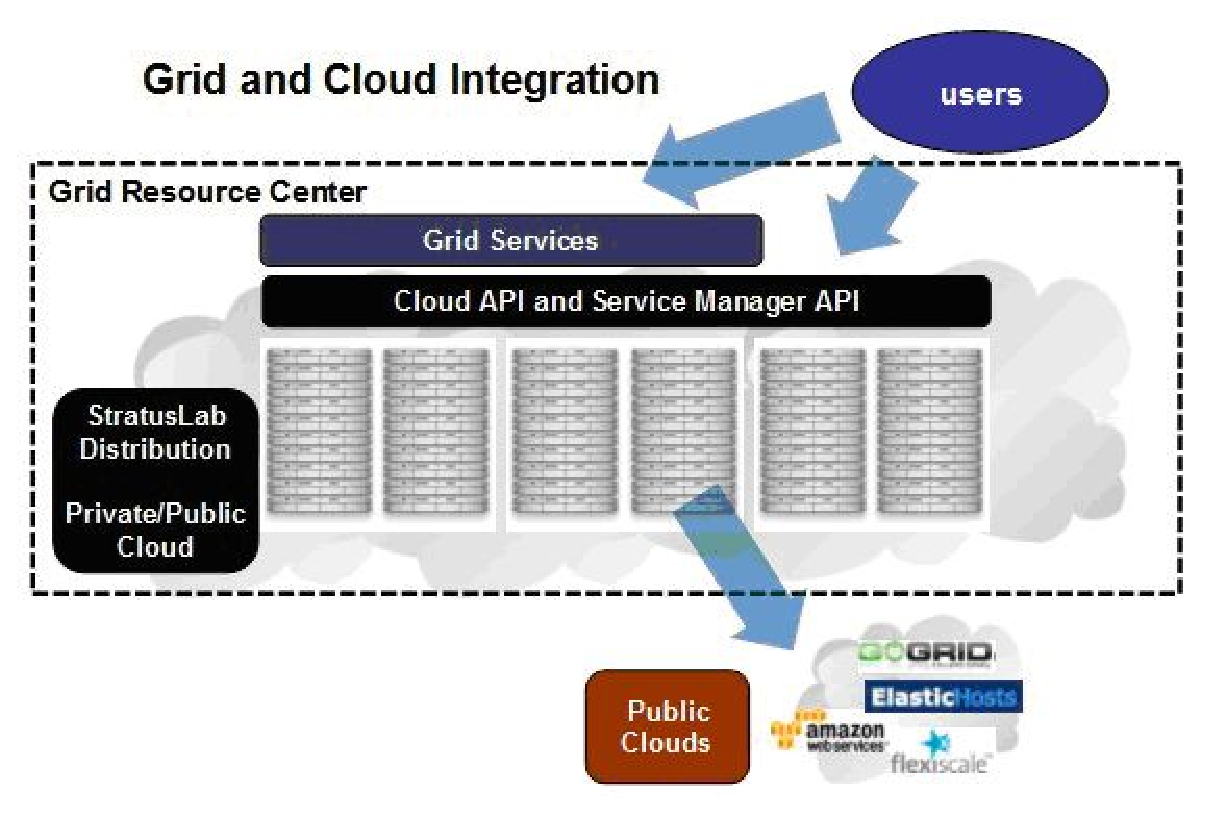
\includegraphics[width=13cm]{fig26.eps} %    ** if .eps don't need extension
\caption{Schema of StratusLab IaaS Cloud interoperability with a
Grid}\label{fig26}
\end{figure}



The basic operations like distributed data management, the high data
throughput and  the remote job submission can probably be more
cloud-like. There is a great interest among people to use commercial
Clouds resources, especially when the experiments see their
resources becoming full.

So, can we use Amazon or Google to do processing of data from LHC?
The point is, one can not be sure what the level of services will be
and what the IN/OUT bandwidth will be. This can in principle be
negotiated with these companies and may bring some level of
agreement. That in principle is doable.

But the preferred and more practical strategy for the future WLCG
development is to deploy over the WLCG resources Cloud interfaces,
managed with high level of virtualization. The Cloud and Grid
interfaces can be deployed in parallel or on top of each other. This
gives a way to evolve into a more standardized infrastructure and
allows to make a transparent use of commercial Clouds.

An example of this architecture is the CERN LXCloud [70] pilot
cluster. Implementation at CERN allows to present a Cloud interface
or to access other public or commercial Clouds. This is happening
with no change to any of the existing Grid services. Another
interesting example is the development of a comprehensive OpenSource
IaaS (Infrastructure as a Service) Cloud distribution within the
StratusLab project [68], see Figure~\ref{fig26}. Anyone can take the
code and deploy it on his site and have IaaS Cloud running on his
site. The project is focused on deploying Grid services on top of
this Cloud, 1) to be a service to existing European Grid
infrastructures and to enable these people to use Cloud-operated
resources and 2) because the developers consider the Grid services
very complex and making sure they run safely on this Cloud should
guarantee that also other applications will run without problems.



\subsection{Concluding remarks}
%
As we already stressed, the WLCG performance during the LHC data
taking in 2009-2011 was excellent and the basic mission of the WLCG
has been fulfilled: the data taking and processing is ongoing
without major show-stoppers, hundreds of people are using the Grid
to perform their analyses and unique scientific results are
delivered within weeks after the data was recorded. In addition, the
experience gained during this data taking ``stress test'' launched new
strategies to be followed on the way of the future WLCG development.
There are fundamental issues like the approaching lack of WLCG
resources and the expansion of new technologies like the Cloud
computing. In the time of writing this paper it looks like we will
see in the future some combination of Grid and Cloud technologies
will be adopted to operate the distributed computing infrastructures
used by the HEP experiments.



%%%%%%%%%%%%%%%%%%%%%%%%%%%%%%%%%%%%%%%%%%%%%%%%%%%%%%%%%%%%%%%%%%%%%%%%%%%%%%%%

\newpage

%%% Without a bib file, write your references like this: **************
\begin{thebibliography}{100}

\bibitem[1]{s1_1}  D.H. Perkins:  Introduction to High Energy Physics, Cambridge
University Press,\\ 4th edition (2000), ISBN-13: 978-0521621960.\\
Procedings of 35th International Conference of High Energy Physics,
July 22-28, 2010, Paris, France,
     Proceedings of Science (PoS) electronic Journal: ICHEP 2010
%
\bibitem[2]{s1_2}  STAR Collaboration: Experimental and theoretical challenges in
the search for the quark gluon plasma: The STAR Collaboration's
     critical assessment of the evidence from RHIC collisions,
     Nucl.~Phys.~A757~(2005)~102-183.
%
\bibitem[3]{s1_3} CERN - the European Organization for Nuclear Research;
\newline\url{http://public.web.cern.ch/public/}
%
\bibitem[4]{s1_4}  The Large Hadron Collider at
CERN; \url{http://lhc.web.cern.ch/lhc/};
\newline\url{http://public.web.cern.ch/public/en/LHC/LHC-en.html}
%
\bibitem[5]{s1_5} ALICE
Collaboration: \url{http://aliceinfo.cern.ch/Public/Welcome.html}
%
\bibitem[6]{s1_6} ATLAS Collaboration: \url{http://atlas.ch/}
%
\bibitem[7]{s1_7}  CMS Collaboration: \url{http://cms.web.cern.ch/}
%
\bibitem[8]{s1_8} LHCb Collaboration: \url{http://lhcb-public.web.cern.ch/lhcb-public/}
%
\bibitem[9]{s1_9} W.N. Cottingham and D.A. Greenwood: An Introduction to the Standard Model of
Particle Physics, Cambridge University Press, 2nd edition (2007), ISBN-13: 978-0521852494
%
\bibitem[10]{s1_10} Worldwide LHC Computing Grid:
\newline\url{http://public.web.cern.ch/public/en/lhc/Computing-en.html}
%
% S2
%
\bibitem[11]{s2_1} LHC Computing Grid: Technical Design Report,
\newline\url{http://lcg.web.cern.ch/LCG/tdr/}
%
\bibitem[12]{s2_2} I. Foster and C. Kesselman. The Grid: Blueprint for a New Computing Infrastructure.
Morgan Kaufmann, 1999;\\
     I. Foster et al: The Anatomy of the Grid: Enabling Scalable Virtual Organizations,
     International Journal of High Performance
     Computing Applications Vol.15(2001), p.200.
%
\bibitem[13]{s2_3} WLCG Memorandum of Understanding,
\newline\url{http://lcg.web.cern.ch/lcg/mou.htm}
%
\bibitem[14]{s2_4} EGI - The European Grid Initiative; \url{http://web.eu-egi.eu/}
%
\bibitem[15]{s2_5} OSG - The Open Science Grid,
\newline\url{http://www.opensciencegrid.org/};
\newline\url{https://osg-ress-1.fnal.gov:8443/ReSS/ReSS-prd-History.html}
%
\bibitem[16]{s2_6} I. Legrand et al: MONARC Simulation Framework, ACAT'04, Tsukuba, Japan,2004;
\newline\url{http://monarc.cacr.caltech.edu:8081/www_monarc/monarc.htm}
%
\bibitem[17]{s2_7} I. Bird: LHC Computing: After the first year with data, TERENA
Networking Conference (TNC2011), Prague, 2011,
       \newline\url{https://tnc2011.terena.org/web/media/archive/7A}
%
\bibitem[18]{s2_8} LHCOPN - The Large Hadron Collider Optical Private Network,
\newline\url{https://twiki.cern.ch/twiki/bin/view/LHCOPN/WebHome}
%
\bibitem[19]{s2_9} The GEANT Project, \url{http://archive.geant.net/}
%
\bibitem[20]{s2_10} USLHCNet: High speed TransAtlantic network for the LHC community,
\newline\url{http://lhcnet.caltech.edu/}
%
% S3
%
\bibitem[21]{s3_3} Virtual Organisation: \url{http://technical.eu-egee.org/index.php?id=147}
%
\bibitem[22]{s3_4} The European Middleware Initiative:
\url{http://www.eu-emi.eu/home}
%
\bibitem[23]{s3_5} The Globus Toolkit: \url{http://www-unix.globus.org/toolkit/}
%
\bibitem[24]{s3_6} OMII - The Open Middleware Infrastructure Institute:
\url{http://www.omii.ac.uk/}
%
\bibitem[25]{s3_7} The Virtual Data Toolkit, \url{http://vdt.cs.wisc.edu/}
%
\bibitem[26]{s3_8} P.~Saiz~et~al.,  AliEn-ALICE environment on the GRID,\\
Nucl.~Instrum.~Meth.~A502~(2003)~437; \url{http://alien2.cern.ch/}
%
\bibitem[27]{s3_9} Computing Element: \url{http://glite.cern.ch/lcg-CE/}
%
\bibitem[28]{s3_10} Workload Management System: \url{http://glite.cern.ch/glite-WMS/}
%
\bibitem[29]{s3_11} The CREAM (Computing Resource Execution And Managemen) Service,
\newline\url{http://glite.cern.ch/glite-CREAM/}
%
\bibitem[30]{s3_12} Storage Element: \url{http://glite.cern.ch/glite-SE_dpm_mysql/}
%
\bibitem[31]{s3_13} dCache: \url{http://www.dcache.org/}
%
\bibitem[32]{s3_14} The Disk Pool Manager:
\newline\url{https://www.gridpp.ac.uk/wiki/Disk_Pool_Manager};
\newline\url{https://twiki.cern.ch/twiki/bin/view/LCG/DataManagementTop}
%
\bibitem[33]{s3_15} XRootD:
\newline\url{http://project-arda-dev.web.cern.ch/project-arda-dev/xrootd/site/index.html}
%
\bibitem[34]{s3_16} SLAC (Stanford Linear Accelerator Center):
\url{http://slac.stanford.edu/}
%
\bibitem[35]{s3_17} INFN - The National Institute of Nuclear Physics:
\newline\url{http://www.infn.it/indexen.php}
%
\bibitem[36]{s3_18} R. Brun and F. Rademakers, ROOT: An object oriented data analysis framework,\\
Nucl.~Instrum.~Meth.~A389~(1997)~81; \url{http://root.cern.ch}
%
\bibitem[37]{s3_19} The VO-box: \url{http://glite.cern.ch/glite-VOBOX/}
%
% S4
%
\bibitem[38]{s4_1} ALICE Experiment Computing TDR:
\newline\url{http://aliceinfo.cern.ch/Collaboration/Documents/TDR/Computing.html}
%
\bibitem[39]{s4_5} CERN Advanced Storage Manager:
\newline\url{http://castor.web.cern.ch/castor/}
%
\bibitem[40]{s4_6} Monitoring Agents using a Large Integrated Services
Architecture:
\newline\url{http://monalisa.cern.ch/monalisa.html};\\
         C.~Grigoras et al., Automated agents for management and control of the ALICE Computing Grid,
         Proceedings of the 17th Int. Conf. CHEP 2009,
         Prague, March 21-27, 2009, J.~Phys.: Conf.~Ser.~219,~062050.
%
\bibitem[41]{s4_7} ALICE raw data production cycles:
\newline\url{http://alimonitor.cern.ch/production/raw.jsp}
%
\bibitem[42]{s4_8} Monitoring of Analysis trains in ALICE:
\newline\url{http://alimonitor.cern.ch/prod/}
%
\bibitem[43]{s4_9} ALICE simulation framework:
\newline\url{http://aliceinfo.cern.ch/Offline/Activities/Simulation/index.html}
%
\bibitem[44]{s4_10} ALICE MC simulation cycles:
\newline\url{http://alimonitor.cern.ch/job_details.jsp}
%
\bibitem[45]{s4_11} AliRoot: \url{http://aliceinfo.cern.ch/Offline/AliRoot/Manual.html}
%
\bibitem[46]{s4_12} GEANT3-Detector Description and Simulation Tool:
\newline\url{http://wwwasd.web.cern.ch/wwwasd/geant/}
%
\bibitem[47]{s4_13} FLUKA-Particle Physics MonteCarlo Simulation package:
\newline\url{http://www.fluka.org/fluka.php}
%
\bibitem[48]{s4_14} Pythia6: \url{http://projects.hepforge.org/pythia6/};\\
Pythia8: \url{http://home.thep.lu.se/~torbjorn/pythiaaux/present.html}
%
\bibitem[49]{s4_15} Xin-Nian Wang and Miklos Gyulassy: HIJING: A Monte Carlo model for
multiple jet production in pp, pA and AA collisions,\\ Phys.~Rev.~D44~(1991),~3501;
         \newline\url{http://www-nsdth.lbl.gov/~xnwang/hijing/}
%
\bibitem[50]{s4_16} ALICE Offline policy:
\newline\url{http://aliceinfo.cern.ch/Offline/General-Information/Offline-Policy.html}
%
\bibitem[51]{s4_17} ALICE Computing sites:
\newline\url{http://pcalimonitor.cern.ch:8889/reports/};\\
ALICE Distributed Storage: \newline\url{http://pcalimonitor.cern.ch/stats?page=SE/table}
%
\bibitem[52]{s4_18} Yves Schutz: Computing resources 2011-2013, ALICE Computing Board
Sept.~1st, 2011:
\newline\url{http://indico.cern.ch/materialDisplay.py?contribId=3&materialId=2&confId=153622};\\
\newline\url{https://twiki.cern.ch/twiki/bin/view/FIOgroup/TsiBenchHEPSPEC}
%
% S5
%
\bibitem[53]{s5_2}  gLite-Lightweight Middleware for Grid Computing,
\newline\url{http://glite.cern.ch/}
%
\bibitem[54]{s5_3}  ARC-The Advanced Resource Connector middleware,
\newline\url{http://www.nordugrid.org/arc/about-arc.html}
%
\bibitem[55]{s5_5} The AliEn Shell-aliensh,
         AliEn User Interfaces:
\newline\url{http://project-arda-dev.web.cern.ch/project-arda-dev/alice/apiservice/guide/guide-1.0.html#_Toc156731986};\\
         ALICE Grid Analysis:
\newline\url{http://project-arda-dev.web.cern.ch/project-arda-dev/alice/apiservice/AA-UserGuide-0.0m.pdf}
%
\bibitem[56]{s5_7}  The PANDA Experiment: \url{http://www-panda.gsi.de/}
%
\bibitem[57]{s5_8} GAS-Grid Access Service in AliEn:
         P. Buncic et al, The architecture of the AliEn system,
         Proc of the Conference on Computing in High Energy Physics and Nuclear Physics
         2004 (CHEP'04), Interlaken, Switzerland,
         \newline\url{http://cdsweb.cern.ch/record/865533/files/p951.pdf}
%
\bibitem[58]{s5_9} VOMS-Virtual Organization Membership Service:
\newline\url{http://glite.web.cern.ch/glite/packages/R3.1/deployment/glite-VOMS_mysql/glite-VOMS_mysql.asp}
%
\bibitem[59]{s5_10} Job statuses in AliEn:
\newline\url{http://pcalimonitor.cern.ch/show?page=jobStatus.html}
%
% S6
%
\bibitem[60]{s6_1} LHC Design Report:
\url{http://lhc.web.cern.ch/lhc/LHC-DesignReport.html}
%
\bibitem[61]{s6_2} LHC Performance and Statistics:
\newline\url{https://lhc-statistics.web.cern.ch/LHC-Statistics/}
%
\bibitem[62]{s6_5} The ALICE Collaboration: First proton-proton
collisions at the LHC as observed with the ALICE detector:
measurement of the charged-particle
        pseudorapidity density at $\sqrt{s}=900$ GeV, Eur.~Phys.~J.~C65~(2010),~111-125.
%
\bibitem[63]{s6_6} Quark Matter 2011: \url{http://qm2011.in2p3.fr/}
%
\bibitem[64]{s6_7} The ALICE
Collaboration: Charged-Particle Multiplicity Density at Midrapidity
in Central Pb-Pb Collisions at $\sqrt{s_{NN}}=2.76$ TeV,
        Phys.~Rev.~Lett.~105~(2010),~252301.
%
\bibitem[65]{s6_8} The ALICE Collaboration: Elliptic Flow of Charged Particles
in Pb-Pb Collisions at $\sqrt{s_{NN}}=2.76$ TeV,
Phys.~Rev.~Lett.~105~(2010),~252302.
%
\bibitem[66]{s6_9} Physics Publications of the ALICE
Collaboration in Refereed Journals,
\newline\url{http://aliceinfo.cern.ch/Documents/generalpublications}
%
% S7
%
\bibitem[67]{s7_1} I. Foster et al: Cloud Computing and Grid Computing
360-Degree Compared, Proc. of the Grid Computing Environments
Workshop, 2008. GCE '08, Austin, Texas,
\newline\url{http://arxiv.org/ftp/arxiv/papers/0901/0901.0131.pdf}
%
\bibitem[68]{s7_2} C. Loomis: StratusLab: Enhancing Grid Infrastructures with
Cloud and Virtualization Technologies, TERENA Networking Conference
(TNC2011),Prague, 2011,
\newline\url{https://tnc2011.terena.org/web/media/archive/11C}
%
\bibitem[69]{s7_3} LHCONE-LHC Open Network Environment:
\newline\url{http://lhcone.net/}
%
\bibitem[70]{s7_5} LXCloud:
\url{https://twiki.cern.ch/twiki/bin/view/FIOgroup/LxCloud}




%\bibitem[Arai \& Kragic, 1999]{arai99} Arai, T. \& Kragic, D. (1999). Name of paper, In: \emph{Name of Book in Italics}, Name(s) of Editor(s), (Ed.), page numbers (first-last), Publisher, ISBN, Place of publication

%\bibitem[Arkin, 2004]{arkin04} Arkin, D. (2004). \emph{My Life}, Arkin Publishing, Arkinson.

%\bibitem[Li et al., 1996]{li96} Li, B.; Xu, Y. \& Choi, J. (1996). Title of conference paper,  \emph{Proceedings of xxx xxx in italics}, pp. 14-17, ISBN, conference location, month and year, Publisher, City

%\bibitem[Lima et al., 2004]{lima04} Lima, P.; Bonarini, A. \& Mataric, M. (2004). \emph{Name of Book in Italics}, Publisher, ISBN, Place of Publication.

%\bibitem[Mataric \& Brooks, 1999]{mataric99} Mataric M. \& Brooks, R. (1999). To whom it may concern. \emph{Journal of Everything}, Vol. $\infty$, No. $\aleph_0$, Jan -1999, -10 -- -5, ISSN 00-XY-A

%\bibitem[Siegwart, 2001]{siegwart01} Siegwart, R. (2001). Name of paper. \emph{Name of Journal in Italics}, Vol., No., (month and year of the edition) page numbers (first-last), ISSN

%\bibitem[Siegwart et al., 2006]{siegwart06} Siegwart, R.; Gross, S.; Klein L. (2006). The Singularity has gone. \emph{Future beyond Science}, Vol. 0, No. 0, April 3000, 1--1 000 000, ISSN 00-0000-00-00Y

\end{thebibliography}

%%% With a bib file, include it! *************************************


\end{document}
